%% ============================================================
%%  Memo – Causal Shapley Values (condensed, ≤10 content pages)
%%  Juan David Rios Garcia
%%  Compile: pdflatex -> bibtex -> pdflatex x2
%% ============================================================
\documentclass[12pt,letterpaper,twocolumn]{article}

%% ── Fonts (Times New Roman) ─────────────────────────────────
\usepackage{newtxtext,newtxmath}
\usepackage[T1]{fontenc}
\usepackage[utf8]{inputenc}
\usepackage{microtype}

%% ── Page geometry ───────────────────────────────────────────
\usepackage[top=2cm, bottom=2cm, left=1.8cm, right=1.8cm]{geometry}

%% ── Spacing ─────────────────────────────────────────────────
\usepackage{setspace}
\singlespacing
\usepackage{parskip}
\setlength{\parskip}{3pt}

%% ── Mathematics ─────────────────────────────────────────────
\usepackage{amsmath}
\usepackage{mathtools}
\usepackage{bm}

%% ── Algorithms ──────────────────────────────────────────────
\usepackage{algorithm}
\usepackage{algpseudocode}
\algnewcommand\algorithmicinput{\textbf{INPUT:}}
\algnewcommand\INPUT{\item[\algorithmicinput]}
\algnewcommand\algorithmicoutput{\textbf{OUTPUT:}}
\algnewcommand\OUTPUT{\item[\algorithmicoutput]}
\algnewcommand\algorithmicprecompute{\textbf{PRECOMPUTE:}}
\algnewcommand\PRECOMPUTE{\item[\algorithmicprecompute]}

%% ── Tables ──────────────────────────────────────────────────
\usepackage{booktabs}
\usepackage{tabularx}
\usepackage{multirow}
\usepackage{array}
\newcolumntype{L}[1]{>{\raggedright\arraybackslash}p{#1}}
\newcolumntype{C}[1]{>{\centering\arraybackslash}p{#1}}
\newcolumntype{R}[1]{>{\raggedleft\arraybackslash}p{#1}}

%% ── Graphics ────────────────────────────────────────────────
\usepackage{graphicx}
\usepackage{float}
\usepackage{subcaption}
\usepackage{caption}
\captionsetup{font=footnotesize, labelfont=bf}

%% ── Colours ─────────────────────────────────────────────────
\usepackage[dvipsnames,table]{xcolor}

%% ── Hyperlinks ──────────────────────────────────────────────
\usepackage[hidelinks, breaklinks=true,
            pdfauthor={Juan David Rios Garcia},
            pdftitle={Evaluating the Impact of Discovered Causal Structures on
                      Structure-Aware Shapley Methods}]{hyperref}

%% ── References ──────────────────────────────────────────────
\usepackage[numbers,sort&compress]{natbib}
\bibliographystyle{plainnat}

%% ── Miscellaneous ───────────────────────────────────────────
\usepackage{enumitem}
\usepackage{fancyhdr}
\pagestyle{fancy}
\fancyhf{}
\fancyhead[R]{\small\nouppercase{\leftmark}}
\fancyfoot[C]{\thepage}
\renewcommand{\headrulewidth}{0.4pt}

%% ── Algorithm name ──────────────────────────────────────────
\makeatletter
\renewcommand{\ALG@name}{Algorithm}
\makeatother

%% ============================================================
\begin{document}
%% ============================================================

%% ── Full-width title + abstract ─────────────────────────────
\twocolumn[{%
  \centering
  {\Large\bfseries Evaluating the Impact of Discovered Causal Structures on\\[0.3em]
  Structure-Aware Shapley Methods: An Experimental Pipeline\par}
  \vspace{0.5em}
  {\normalsize Juan David Rios Garcia \quad 2026\par}
  \vspace{0.8em}
  \begin{minipage}{0.95\linewidth}
    \small\textbf{Abstract.}
    Structure-aware Shapley methods promise more faithful feature attributions by
    embedding causal graph topology into the credit-assignment process. In practice
    the causal graph is rarely known: practitioners must infer it from data using
    automated discovery algorithms whose outputs are noisy and error-prone. This
    paper introduces an experimental pipeline that feeds automatically discovered
    graphs (PC and DirectLiNGAM) into three structure-aware methods, Asymmetric
    Shapley (ASV), Causal Shapley (CSV), and Shapley Flow, and measures attribution
    quality degradation along two dimensions: Magnitude Divergence ($\Delta M$) and
    Sign Disagreement ($D$), each against three reference configurations. Experiments
    on a 50-feature confounded synthetic dataset and the Sachs cell-signaling
    benchmark show that ASV is the most stable under graph errors( both $\Delta M_{\text{oracle}}$
    and $D_{\text{oracle}}$ are the lowest divergence in all comparisons), while CSV and Flow amplify
    discovery errors into large attribution shifts. The pipeline also provides a
    dual-signal diagnostic, based on joint $\Delta M_{\text{base}}$ and
    $\Delta M_{\text{disc}}$, standardized metrics, that identifies structurally unreliable nodes without
    needing a ground-truth graph, and adapt to any dataset and model output dimensions.
  \end{minipage}
  \vspace{0.8em}
  \hrule
  \vspace{0.6em}
}]

%% ============================================================
\section{Introduction}
\label{sec:intro}
%% ============================================================

Explainable AI has moved from a research preference to a deployment requirement across
critical decisioning domains such as credit scoring, healthcare, and public resource allocation,
where model decisions must be justified to affected individuals and regulatory bodies
\citep{Baron2023}. Shapley values have emerged as a gold standard for local feature
attribution, but traditional implementations assume feature independence, which in practice means treating all
permutations as equally probable during coalition formation, or just sampling marginal distributions when they are correlated, 
this could give a false credit when the true generative process involves causal dependencies among
inputs \citep{Lundberg2017, Heskes2020}.

Recent literature has introduced structure-aware Shapley frameworks that embed causal
graph topology into the attribution process or modify the sampling strategy to capture dependencies.
Asymmetric Shapley Values (ASV) restrict permutations to causal orderings \citep{Frye2021};
Causal Shapley Values (CSV) replace observational marginalization with Pearl's do-calculus \citep{Heskes2020};
and Shapley Flow reframes credit assignment from nodes to directed edges \citep{Wang2021}. All three
promise attributions more faithful to the underlying causal mechanism, but every one of
these methods treats the causal graph as given.

In practice the graph is almost never directly observable: practitioners must rely on
automated discovery algorithms such as the PC algorithm \citep{Spirtes2000} and
DirectLiNGAM \citep{Shimizu2011} to infer it from observational data. These estimated
graphs are inherently noisy, subject to false-positive and false-negative edge errors,
and sensitive to assumption violations \citep{Glymour2019}.

We build an experimental pipeline that feeds automatically discovered graphs into the
three methods and measures, for the first time, how much attribution quality degrades
when the graph is imperfect. Evaluation is performed on a controlled synthetic dataset
(50 features, known linear causal structure) and the real-world Sachs cell-signaling
dataset \citep{Sachs2005}, where an established consensus DAG allows external
validation.

To answer the central question consistently we track two dimensions: the \emph{magnitude}
of the attribution assigned to a feature and the \emph{sign} (direction) of that
attribution. A graph that merely rescales attributions preserves the qualitative story
told to an affected individual; a graph that inverts signs tells the opposite story.
Each dimension is operationalized by a single metric used identically across three
comparison configurations (vs.\ baseline, vs.\ oracle, and cross-discovery), establishing
a universal diagnostic framework.

%% ============================================================
\section{Conceptual Framework}
\label{sec:framework}
%% ============================================================

\subsection{Explaining Models, Not Nature}

One distinction matters before going any further, the goal here is not to fully recover the
physical laws of the system the model was trained on, but to capture enough of its
causal structure to make the attribution computation more honest \citep{Baron2023}.
A practitioner does not need a complete causal model of the world; they need a
plausible graph of how the input features relate to each other so that structure-aware
methods can encode those relationships as constraints, rather than treating every feature
as an independent, interchangeable partner. Physical interventions are not required and
often not possible; what matters is that the graph reflects the real dependencies well
enough to guide the credit-assignment process in the right direction.

\subsection{Structural Causal Models and Credit Attribution}

A Structural Causal Model (SCM) \citep{Pearl2009} describes a system as a set of
equations $x_i = f_i(\mathrm{Pa}(x_i), \varepsilon_i)$ where each variable is determined
by its causal parents and independent noise. When a full SCM is available, credit
attribution becomes more precise: you can intervene on a variable, fixing it to a
specific value while cutting its incoming edges, and trace how that change propagates
through the graph to the final prediction. This is the intuition behind CSV and Shapley
Flow, both of which are designed around this causal intervention idea. CSV approximates
the post-interventional distribution using Pearl's do-operator for each coalition
evaluation; Flow routes credit along the actual graph edges so that structural paths
determine how much each node contributes. In practice, a fully specified SCM is almost
never available. The implementations here do not reconstruct structural equations: CSV
uses a conditional Gaussian approximation along discovered parent sets, and Flow uses
a binary foreground/background activation rule. Both methods still benefit from the
graph topology, but the credit assignment is an approximation of the full interventional
ideal rather than an exact application of it.

\subsection{Causal Discovery}

Two prominent discovery algorithms accessible to any practitioner are used in this
pipeline.Both algorithms operate on the $X$-only training partition.

\paragraph{PC \citep{Spirtes2000}.} A constraint-based method that recovers the causal
skeleton through conditional independence tests (Fisher-z, $\alpha = 0.05$) and applies
Meek's orientation rules. Undirected edges are resolved by orienting them from lower to
higher feature index.

\paragraph{DirectLiNGAM \citep{Shimizu2011}.} A functional causal model that exploits
linear non-Gaussian structures to simultaneously identify causal ordering and structural
coefficients. Edges with $|\text{coefficient}| < 0.10$ are pruned. 

\subsection{Traditional Shapley Values}

Shapley values originate in cooperative game theory as the unique fair allocation of
total payoff among players \citep{Shapley1953}. The marginal contribution of feature $i$
to coalition $S$ is $v(S \cup \{i\}) - v(S)$, where $v(S) = \mathbb{E}[f(X) \mid X_S =
x_S]$. Averaging over all orderings gives:
\begin{equation}
  \phi_i = \!\sum_{S \subseteq N \setminus \{i\}} \frac{|S|!\,(|N|-|S|-1)!}{|N|!}
  \bigl[ v(S \cup \{i\}) - v(S) \bigr].
\end{equation}
The formula is the unique solution satisfying four axioms: \textit{Efficiency}
(attributions sum to the total model output minus the baseline); \textit{Null Player}
(a feature that never changes the coalition value receives zero credit); \textit{Linearity}
(attributions for a weighted sum of games equal the weighted sum of their attributions);
and \textit{Symmetry} (two features with identical marginal contributions to every
coalition receive equal attribution). Together these axioms guarantee a principled,
unambiguous allocation: no matter how complex the model, the credit is divided exhaustively,
no player is penalized for doing nothing, and identical contributions earn identical
rewards. Symmetry is especially important for its fairness interpretation, it prevents
arbitrary tie-breaking and ensures that attribution differences reflect genuine
differences in predictive contribution rather than the order in which features were
considered.

Where Symmetry becomes problematic is when the input features are not, in fact,
interchangeable. If $X_i$ is a causal parent of $X_j$, treating them as symmetric
partners means the uniform average over orderings includes orderings where $X_j$ appears
before $X_i$, orderings that reverse the real generative sequence. These orderings let
$X_j$ absorb credit that, causally, belongs to $X_i$, because in the true data-generating
process $X_j$'s values are partly determined by $X_i$. The result is a systematic
misattribution from upstream causes to downstream effects whenever features are correlated
through causal structure.

\subsection{Structure-Aware Methods}

All three methods preserve Efficiency, Linearity, and Null Player while modifying
Symmetry to accommodate causal topologies.

\paragraph{Asymmetric Shapley (ASV).} Replaces the uniform distribution over orderings
with a distribution placing mass only on topological orderings of the feature DAG
\citep{Frye2021}:
\begin{equation}
  \phi_i(\mathrm{ASV}) = \mathbb{E}_{\pi \sim U(\Pi_{\mathrm{topo}})}
  \bigl[ v(P_i^\pi \cup \{i\}) - v(P_i^\pi) \bigr].
\end{equation}
The coalition value remains observational; the graph enters only through the permutation
set $\Pi_{\mathrm{topo}}$.

\paragraph{Causal Shapley (CSV).} Keeps the symmetric formulation but replaces the
observational value function with an interventional one based on Pearl's do-operator
\citep{Heskes2020}:
\begin{equation}
  v_{\mathrm{do}}(S) = \mathbb{E}[f(X) \mid \mathrm{do}(X_S = x_S)].
\end{equation}
CSV uses $v_{\mathrm{do}}$ in the standard Shapley weighting formula. The interventional
value is estimated by post-interventional sampling along the graph-defined parent sets
using a conditional Gaussian approximation (Appendix~\ref{app:algorithms}).

\paragraph{Shapley Flow.} Moves from node-based to edge-based attribution
\citep{Wang2021}. The players are the directed graph edges:
\begin{equation}
  \phi_{u \to v} = \mathbb{E}_{\pi \sim U(\Pi_E)}
  \bigl[ V(E_{u \to v}^\pi \cup \{u \to v\}) - V(E_{u \to v}^\pi) \bigr],
\end{equation}
and node importance is $\phi_u = \sum_{v:\, u \to v \in E} \phi_{u \to v}$. Each node
takes its foreground value if it has any active incident edge; otherwise its background
value. With no graph there is no game to play.

%% ============================================================
\section{Experimental Setup}
\label{sec:setup}
%% ============================================================

\begin{figure*}[tp]
  \centering
  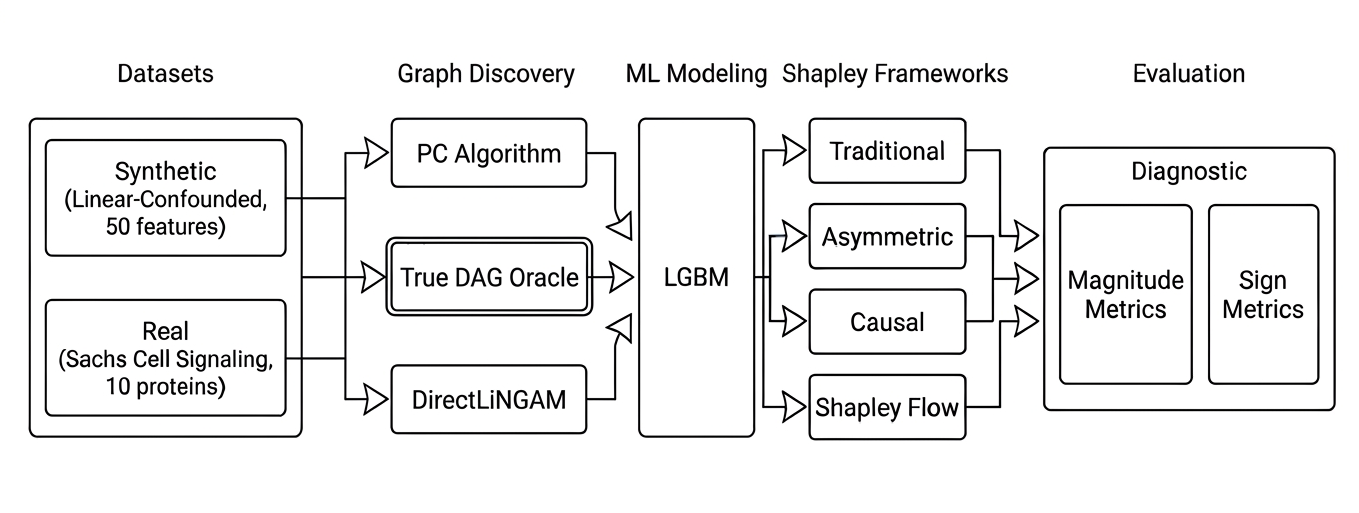
\includegraphics[width=\linewidth]{figures/experimental_pipeline_diagram.png}
  \caption{\textbf{Experimental pipeline overview.} End-to-end flow from data
  generation and causal discovery through Shapley computation to evaluation, showing
  how the two datasets, three graph sources, and three structure-aware methods feed
  into the magnitude and sign metrics.}
  \label{fig:pipeline}
\end{figure*}

Figure~\ref{fig:pipeline} shows the end-to-end experimental pipeline. Two datasets are evaluated
across three structure-aware Shapley methods under three causal graph sources; the
resulting attributions are measured along magnitude and sign dimensions.

\subsection{Datasets}

\paragraph{Synthetic (Linear-Confounded).}
Strictly linear structural equations $X_j = \sum_{i \in \mathrm{Pa}(j)} w_{ij} X_i +
\varepsilon_j$ ($\varepsilon_j \sim \mathcal{N}(0, 0.5)$, coefficients $\in
\mathrm{Uniform}(0.5, 2.0)$). Erd\H{o}s--R\'{e}nyi graph ($p = 0.07$, 87 $X \to X$
edges, 50 features, 15 direct parents of $Y$). Five hidden confounders each influence
2--3 features, creating a noisy scenario for both discovery algorithms. 1000 observations.

\paragraph{Sachs Cell Signaling \citep{Sachs2005}.}
7,466 simultaneous measurements of 11 protein concentrations in stimulated human
T-cells. Akt (\texttt{akt}) is the regression target; 10 proteins are input features.
A consensus reference DAG (17 $X \to X$ edges, 3 direct $X \to Y$ edges) provides
oracle ground truth. Preprocessing: log1p transformation, then a Standard Scaler fit
on the training partition only. Both datasets use an 80/20 split, seed 42.

\subsection{Predictive Model}

LightGBM regressor fitted with Optuna hyperparameter optimization (50 TPE trials,
RMSE objective). Feature selection is disabled so all features participate in the
Shapley computation. Table~\ref{tab:model_performance} reports performance; $\hat{\sigma}$
is the standard deviation of model predictions over the test set and normalizes all
magnitude metrics; the normalization rationale is explained in Section~\ref{sec:metrics}.

\begin{table}[H]
  \centering
  \footnotesize
  \caption{\textbf{Model performance.} $\hat{\sigma}$ normalizes all $\Delta M$ metrics.}
  \label{tab:model_performance}
  \begin{tabular}{lrrrr}
    \toprule
    \textbf{Dataset} & \textbf{R\textsuperscript{2}} & \textbf{RMSE} & \textbf{MAE} & $\hat{\sigma}$ \\
    \midrule
    Synthetic & 0.900 & 1.72  & 1.36  & 4.71  \\
    Sachs     & 0.679 & 88.78 & 17.82 & 116.76  \\
    \bottomrule
  \end{tabular}
\end{table}

\subsection{Discovery and Computation Settings}

Both discovery algorithms are configured as described in Section~\ref{sec:framework}.
Because neither algorithm produces $X \to Y$ edges,
an augmentation step appends direct $X_i \to Y$ edges for every feature, uniformly
applied to the True DAG as well, guaranteeing Shapley Flow has a route to accumulate
credit for every node.

All Shapley methods use Monte Carlo approximation with $T = 100$ permutations. Background
reference: 30\% of training rows (240 synthetic; 1,791 Sachs). Up to 100 test instances
explained. CSV uses $M = 10$ inner interventional samples per coalition. Table~\ref
{tab:method_comparison} summarizes what each method changes relative to Traditional
Shapley.

\begin{table}[H]
  \centering
  \footnotesize
  \setlength{\tabcolsep}{3pt}
  \caption{\textbf{What each method changes relative to Traditional Shapley.}}
  \label{tab:method_comparison}
  \begin{tabularx}{\columnwidth}{p{1.3cm}XXXX}
    \toprule
    \textbf{Prop.} & \textbf{Trad.} & \textbf{ASV} & \textbf{CSV} & \textbf{Flow} \\
    \midrule
    Players    & Features & Features    & Features    & Edges \\
    Perms.     & $N!$ ord. & Restricted & Restricted  & $|E|{+}1$ \\
    Value fn.  & Obs.     & Obs.        & Intervent.  & Fg/bg act. \\
    Graph role & None     & Ordering    & Order+cond. & Players \\
    \bottomrule
  \end{tabularx}
\end{table}

\subsection{Evaluation Metrics}
\label{sec:metrics}

Every comparison asks two questions about a (method, graph) result against a reference:
did the attribution change in \textbf{magnitude}, and did it change in \textbf{direction}?
Let $\phi^{m,G}_{i,f}$ be the Shapley value for feature $f$, instance $i$, method $m$,
graph $G$.

\paragraph{Magnitude Divergence ($\Delta M$).}
At instance level, the signed gap between attribution magnitudes is
$\delta^{\mathrm{ref}}_{i,f} = |\phi^{m,G}_{i,f}| - |\phi^{\mathrm{ref}}_{i,f}|$.
Squaring and averaging over all explained instances $\mathcal{I}$ gives a
feature-level root-mean-square divergence, then divided by $\hat{\sigma}$:
\begin{equation}
  \Delta M^{\mathrm{ref}}_f =
  \frac{1}{\hat{\sigma}}\sqrt{\frac{1}{|\mathcal{I}|}
  \sum_{i \in \mathcal{I}} \!\left(\delta^{\mathrm{ref}}_{i,f}\right)^2}.
\end{equation}
The global dataset-level score averages across all $N$ features:
$\Delta M^{\mathrm{ref}} = \frac{1}{N}\sum_f \Delta M^{\mathrm{ref}}_f$.

The denominator $\hat{\sigma}$ is the standard deviation of model predictions over the
test set (reported in Table~\ref{tab:model_performance}). Dividing by $\hat{\sigma}$
expresses every divergence as a fraction of the model's own output spread, making the
numbers directly comparable across datasets, models, and output units. A value of
$\Delta M = 0.10$ means the typical attribution shift for that feature equals 10\% of
the model's prediction spread, regardless of whether the model outputs loan amounts in
thousands of dollars or protein concentrations in arbitrary units. Without this
normalization, the synthetic and Sachs numbers ($\hat{\sigma} = 4.71$ vs.\ $116.76$)
would be on completely different scales and no comparison would be meaningful.

The feature-level view ($\Delta M^{\mathrm{ref}}_f$) is what drives the case studies
in Section~\ref{sec:cases}: it isolates which specific nodes are most destabilized by
graph errors. The dataset-level view ($\Delta M^{\mathrm{ref}}$) is what drives the
scatter-plot comparisons in Sections~\ref{sec:baseline}--\ref{sec:disc_analysis}.

\paragraph{Sign Disagreement ($D$).}
The fraction of (instance, feature) pairs where the attribution flips sign relative to
the reference. $D \in [0, 1]$; $D = 0$ means every attribution points in the same
direction as the reference; $D = 0.33$ means one in three attributions is inverted.
Sign flips are qualitatively more damaging than magnitude shifts: a rescaled attribution
still tells the same directional story to an affected individual; an inverted one tells
the opposite story.

\paragraph{Three reference configurations.}
The same two metrics are computed against three different references, each answering a
distinct practical question:

\begin{itemize}[nosep, leftmargin=1em]
  \item \textbf{vs.\ Traditional ($\Delta M_{\text{base}}$, $D_{\text{base}}$):}
  How much does injecting \emph{any} causal graph change attributions relative to the
  graph-free baseline? A large value here means the method is structurally sensitive to
  the graph: it is doing a lot of additional work beyond standard Shapley. Results in
  Section~\ref{sec:baseline}.

  \item \textbf{vs.\ Oracle ($\Delta M_{\text{oracle}}$, $D_{\text{oracle}}$):}
  How far does a discovered graph push attributions from what the True (or consensus)
  DAG would have produced? This measures the cost of graph imperfection directly.
  Requires a ground-truth graph, so it is only available in controlled settings.
  Results in Section~\ref{sec:oracle_align}.

  \item \textbf{PC vs.\ LiNGAM ($\Delta M_{\text{disc}}$, $D_{\text{disc}}$):}
  How much do attributions change when the same method is fed two different discovered
  graphs from the same data? No ground truth is needed---this is a purely
  observational stability check available to any practitioner. Results in
  Section~\ref{sec:disc_analysis}.
\end{itemize}

Only the \textit{base} and \textit{disc} metrics are available in a real deployment
(oracle requires a known ground-truth graph). The oracle metrics are included here
because the controlled experimental setting allows validating the practical diagnostics
against a known reference.

%% ============================================================
\section{Results and Empirical Analysis}
\label{sec:results}
%% ============================================================

\subsection{Causal Discovery Performance}
On the synthetic track, PC outperforms LiNGAM (F1: 0.567 vs.\ 0.250): conditional independence
tests partially block confounder-induced paths, while LiNGAM's functional model
conflates them with direct paths, adding 81 false-positive edges. On Sachs the ranking
reverses (F1: LiNGAM 0.326 vs.\ PC 0.167): log-transformed proteins retain non-Gaussian
marginals that LiNGAM exploits, while PC's Fisher-z test loses discriminative power
when the massive sample size makes it hypersensitive to distributional violations
\citep{Glymour2019}. Both algorithms perform substantially worse on the real data
despite the larger sample size.

\begin{figure}[H]
  \centering
  
\includegraphics[width=0.85\linewidth]{figures/discovery_vs_r2.png}
  \caption{\textbf{Causal discovery F1 ($X \to X$ edges) versus LightGBM test R\textsuperscript{2}, synthetic vs.\ Sachs.} Bars give PC and LiNGAM F1 on each dataset; the dashed line tracks model R\textsuperscript{2}. The discovery-quality ordering of the two algorithms reverses between tracks even as model fit declines from synthetic to real data.}
  \label{fig:discovery_r2}
\end{figure}

\subsection{Graph-Free Baseline Deviation}
\label{sec:baseline}

This evaluation block compares each structure-aware method and discovered-graph
combination against the Traditional Shapley baseline ($\Delta M_{\text{base}}$,
$D_{\text{base}}$) to verify the expected theoretical behaviour of each method and
validate that this behaviour holds on real data. The theoretical sensitivity ordering
is driven by how deeply each method couples to the graph: ASV uses discovered edges
only to restrict the permutation space while keeping the observational value function
unchanged, so its baseline deviation depends entirely on how many orderings the graph
forbids; CSV is more sensitive because the graph enters the value function itself,
driving post-interventional distributions via discovered parent sets; and Flow is the
most sensitive because the edges are the players of the game, so any graph error
propagates across all downstream paths simultaneously.

Full numeric tables are in Appendix~\ref{app:tables}; scatter plots in
Figure~\ref{fig:scatter_trad}; feature-level magnitude and sign heatmaps in
Appendix~\ref{app:heatmaps_magnitude}--\ref{app:heatmaps_sign}. Two patterns hold across both datasets. First, sign
disagreement $D_{\text{base}}$ is more severe than magnitude divergence
$\Delta M_{\text{base}}$: injecting a causal graph flips the direction of a larger share
of attributions than it inflates their size, because sign inversions arise whenever a
change crosses zero and many near-zero attributions sit close to that threshold. Second,
the choice between PC and LiNGAM barely matters for the graph-versus-no-graph contrast:
both discovered graphs produce nearly identical $\Delta M_{\text{base}}$ and
$D_{\text{base}}$ for a given Shapley method, so the dominant driver is the method's
structural coupling to any graph, not the specific graph supplied.

\textbf{ASV} deviates the least from the Traditional baseline. On synthetic:
$D_{\text{base}} = 5.08$--$5.76\%$, $\Delta M_{\text{base}} = 0.68$--$0.86\%$. On Sachs:
$D_{\text{base}} = 16.80$--$17.00\%$, $\Delta M_{\text{base}} = 4.41$--$5.08\%$. The
larger Sachs numbers reflect its compact 10-node network where each ordering constraint
binds more feature pairs. \textbf{CSV} changes the sign of roughly a third of all
attributions ($D_{\text{base}} \approx 33$--$35\%$ on synthetic, $\approx 31$--$33\%$ on
Sachs). \textbf{Flow} shows the highest magnitude deviation
($\Delta M_{\text{base}}$ up to 14.17\% of $\hat{\sigma}$ on Sachs) and the highest sign
instability on synthetic ($D_{\text{base}} = 36.58$--$37.68\%$).

\begin{figure}[tp]
  \centering
  \begin{subfigure}[t]{0.48\linewidth}
    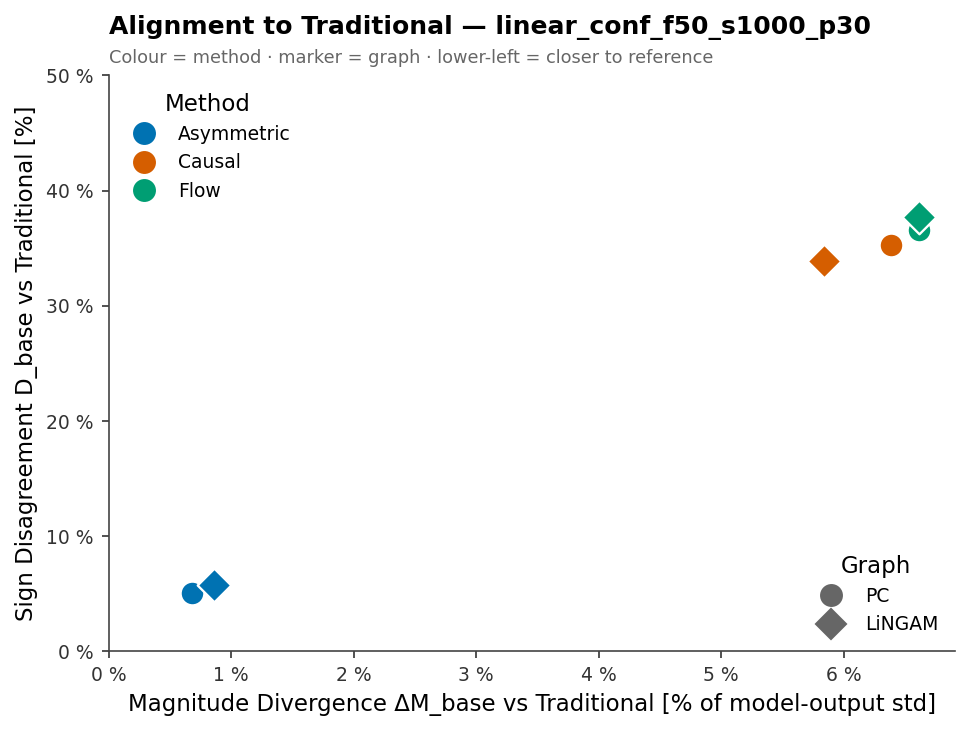
\includegraphics[width=\linewidth]{figures/tga_sa_scatter_traditional_linear_conf_f50_s1000_p30.png}
    \caption{Synthetic.}
    \label{fig:scatter_trad_synth}
  \end{subfigure}
  \hfill
  \begin{subfigure}[t]{0.48\linewidth}
    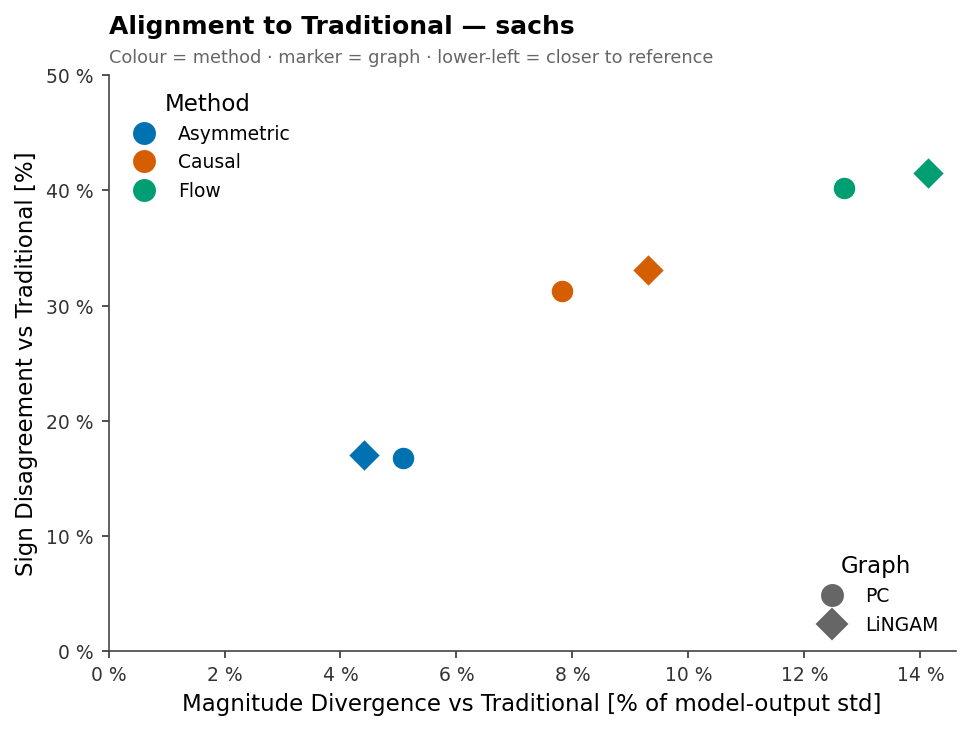
\includegraphics[width=\linewidth]{figures/tga_sa_scatter_traditional_sachs.png}
    \caption{Sachs.}
    \label{fig:scatter_trad_sachs}
  \end{subfigure}
  \caption{\textbf{Deviation from Traditional Shapley.} ASV clusters lower-left;
  CSV and Flow upper-right on both axes. Sachs spreads wider.}
  \label{fig:scatter_trad}
\end{figure}

\subsection{Oracle Alignment}
\label{sec:oracle_align}

Oracle-alignment measures how closely each (method, discovered graph) recovers the
attributions that would be obtained with the True DAG (tables: Appendix~\ref{app:tables};
scatter: Figure~\ref{fig:scatter_oracle}; feature-level heatmaps:
Appendix~\ref{app:heatmaps_magnitude}--\ref{app:heatmaps_sign}). A consistent pattern emerges: the discovery algorithm
with better F1 produces smaller oracle deviation on both dimensions. On synthetic, CSV
under PC (F1 = 0.567) reaches $D_{\text{oracle}} = 31.60\%$, $\Delta M_{\text{oracle}}
= 5.32\%$ vs.\ 37.46\%, 7.57\% under LiNGAM (F1 = 0.250). On Sachs the ranking
reverses: ASV under LiNGAM (F1 = 0.326) achieves $D_{\text{oracle}} = 23.40\%$,
$\Delta M_{\text{oracle}} = 2.84\%$ vs.\ 24.26\%, 9.16\% under PC (F1 = 0.167). Even
imperfect graphs help when they are the better of the two available options.

\textbf{ASV} achieves near-perfect oracle fidelity on synthetic
($\Delta M_{\text{oracle}} < 1.1\%$, $D_{\text{oracle}} < 6.3\%$) regardless of which
discovered graph is supplied. The 81 LiNGAM false-positive edges minimally affect ASV
because in a 50-node sparse system the true and discovered graphs share most valid
topological orderings. \textbf{CSV and Flow} show substantial vulnerability: CSV+LiNGAM
yields $D_{\text{oracle}} = 37.46\%$ and $\Delta M_{\text{oracle}} = 7.57\%$ on
synthetic; Flow shows the largest sign disagreement ($D_{\text{oracle}} = 42.26$--$44.91\%$
on synthetic), meaning close to half of all attributions in all explained features point
in the wrong direction relative to the True DAG.

\begin{figure}[tp]
  \centering
  \begin{subfigure}[t]{0.48\linewidth}
    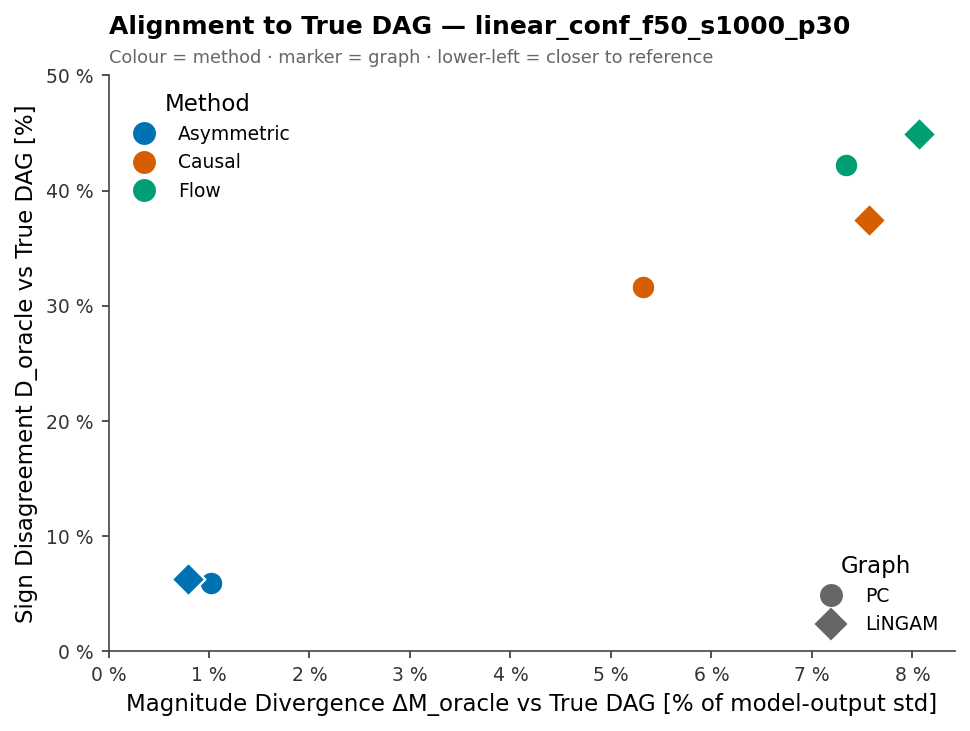
\includegraphics[width=\linewidth]{figures/tga_sa_scatter_true_linear_conf_f50_s1000_p30.png}
    \caption{Synthetic.}
    \label{fig:scatter_oracle_synth}
  \end{subfigure}
  \hfill
  \begin{subfigure}[t]{0.48\linewidth}
    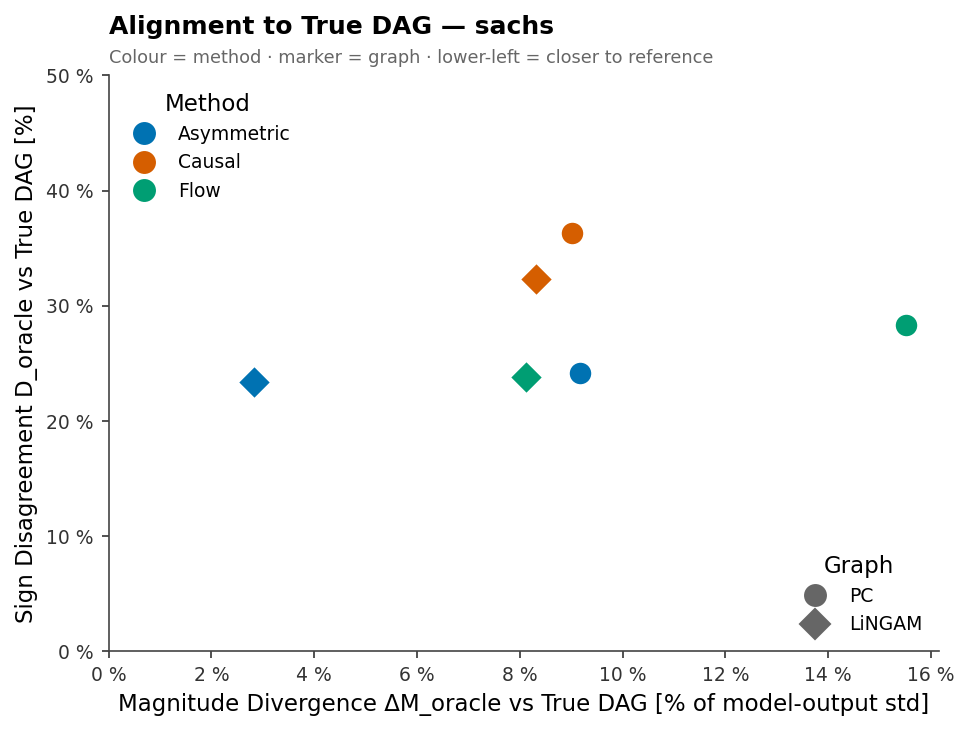
\includegraphics[width=\linewidth]{figures/tga_sa_scatter_true_sachs.png}
    \caption{Sachs.}
    \label{fig:scatter_oracle_sachs}
  \end{subfigure}
  \caption{\textbf{Deviation from the oracle DAG.} ASV lower-left under both
  graphs; CSV and Flow upper-right. PC/LiNGAM markers spread wider on Sachs.}
  \label{fig:scatter_oracle}
\end{figure}

\subsection{Cross-Discovery Sensitivity}
\label{sec:disc_analysis}

If a practitioner runs PC and LiNGAM on the same data and feeds each graph into the
same Shapley method, how much do the explanations change? (Tables:
Appendix~\ref{app:tables}; scatter: Figure~\ref{fig:scatter_disc}; feature-level
heatmaps: Appendix~\ref{app:heatmaps_magnitude}--\ref{app:heatmaps_sign}.) The answer depends heavily on the Shapley method. On Sachs,
Flow's magnitude divergence between the two graphs ($\Delta M_{\text{disc}} = 14.92\%$
of $\hat{\sigma}$) is nearly double ASV's (8.46\%), meaning the choice of discovery
algorithm alone makes Flow attributions twice as volatile. On the sign axis, switching
from ASV to CSV on Sachs determines whether swapping graphs flips 18.60\% or 31.80\%
of attribution signs. With this measures, a practitioner now can have a quantitative expectation
of how much their attributions might change if they had used a different discovery algorithm,
and decide whether that level of instability is acceptable for their use case, and spot possible
sources of divergence, by looking at these metrics a more granular level.

\textbf{ASV} shows the lowest cross-discovery sensitivity on both tracks. On synthetic:
$\Delta M_{\text{disc}} = 1.07\%$, $D_{\text{disc}} = 5.93\%$. On Sachs sensitivity
increases ($\Delta M_{\text{disc}} = 8.46\%$, $D_{\text{disc}} = 18.60\%$) as the compact
network makes different edge sets impose materially different topological constraints.
\textbf{CSV} carries the largest sign instability ($D_{\text{disc}} = 37.94\%$ synthetic,
$31.80\%$ Sachs): interventional conditioning inverts attribution signs whenever parent
sets differ between graphs. \textbf{Flow} carries the largest magnitude instability on
Sachs ($\Delta M_{\text{disc}} = 14.92\%$).

\begin{figure}[tp]
  \centering
  \begin{subfigure}[t]{0.48\linewidth}
    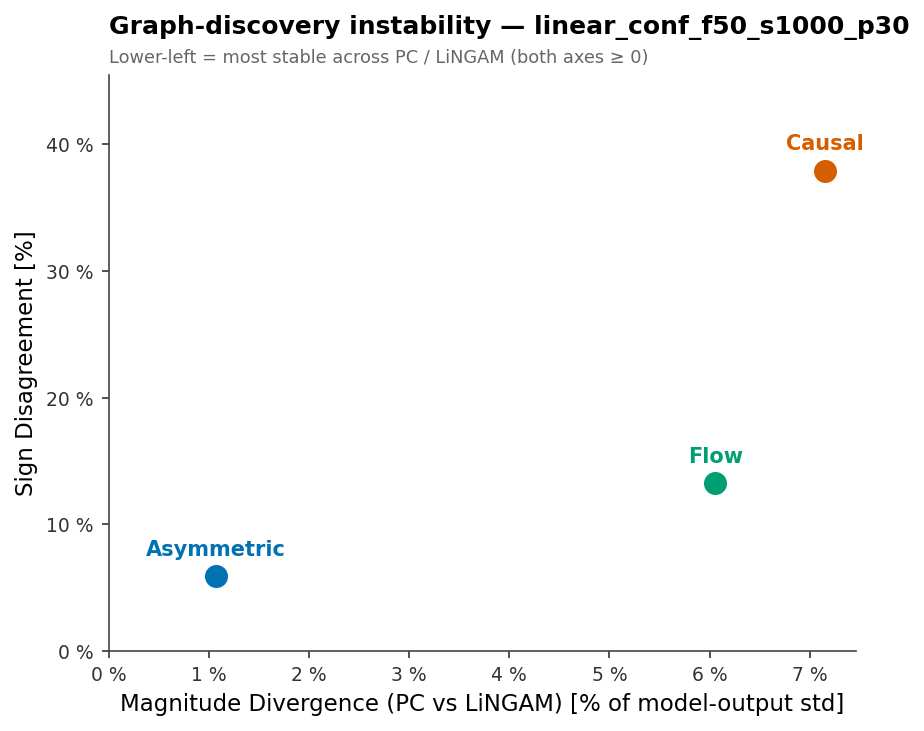
\includegraphics[width=\linewidth]{figures/gss_sss_scatter_linear_conf_f50_s1000_p30.png}
    \caption{Synthetic.}
    \label{fig:scatter_disc_synth}
  \end{subfigure}
  \hfill
  \begin{subfigure}[t]{0.48\linewidth}
    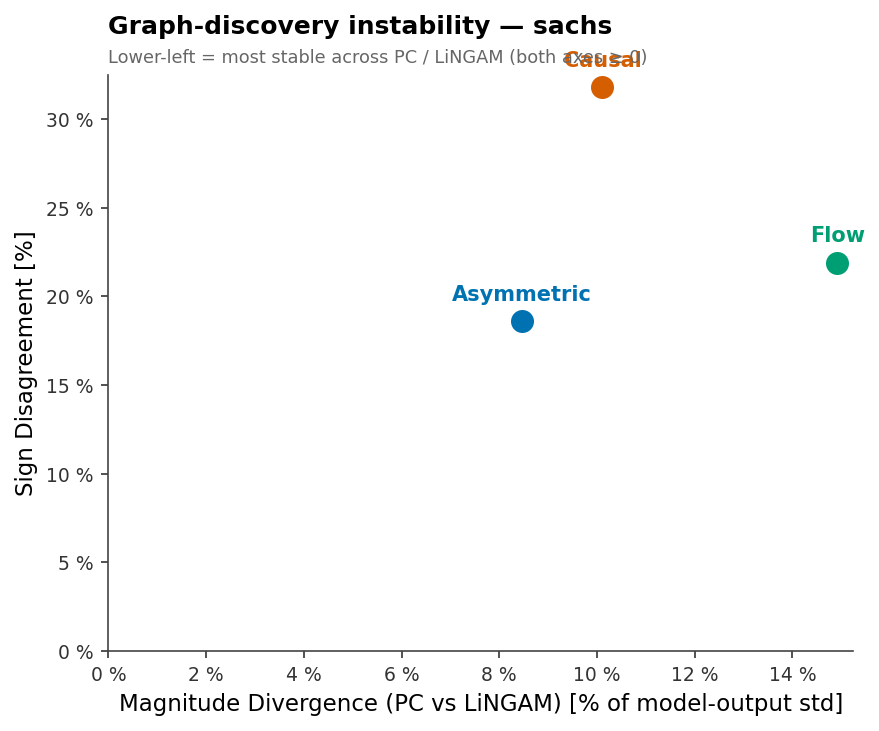
\includegraphics[width=\linewidth]{figures/gss_sss_scatter_sachs.png}
    \caption{Sachs.}
    \label{fig:scatter_disc_sachs}
  \end{subfigure}
  \caption{\textbf{Cross-discovery instability (PC vs.\ LiNGAM).} ASV lower-left
  (stable); CSV upper-right (unstable signs); Flow largest magnitude gap on Sachs.}
  \label{fig:scatter_disc}
\end{figure}

\subsection{Case Studies: When Graph Errors Matter Most}
\label{sec:cases}

Three archetypal error mechanisms illustrate the micro-level behaviour observed across
both experimental tracks. Each is identified by tracing a large global or feature-level
metric back to a specific discovery error.

\subsubsection{Out-Degree Inflation and Root Cause Overloading}

Interventional (CSV) and edge-routing (Shapley Flow) methods over-inflate the attribution of any node that
a discovered graph misrepresents as a high-degree root source. The clearest synthetic
case is X24, a true direct parent of $Y$ with 3 incoming and 4 outgoing edges in the
True DAG. Both PC and LiNGAM strip its true parents and add spurious children
(Figure~\ref{fig:dag_X24}), recasting it as an apparent high-degree root source; this
inflates its outgoing-edge credit under Flow and its interventional parent set under
CSV. X24's feature-level $\Delta M_{\text{base}}$ reaches 32.5\% of $\hat{\sigma}$,the
highest on the synthetic track,and the SHAP scatter (Figure~\ref{fig:shap_X24})
confirms that both discovered-graph columns diverge substantially from the True-DAG
oracle, with inflated and partially sign-flipped values. Any feature producing a
$\Delta M_{\text{base}}$ well above the dataset average deserves scrutiny of its
discovered connections before any Flow attribution is used downstream.

\begin{figure}[H]
  \centering
  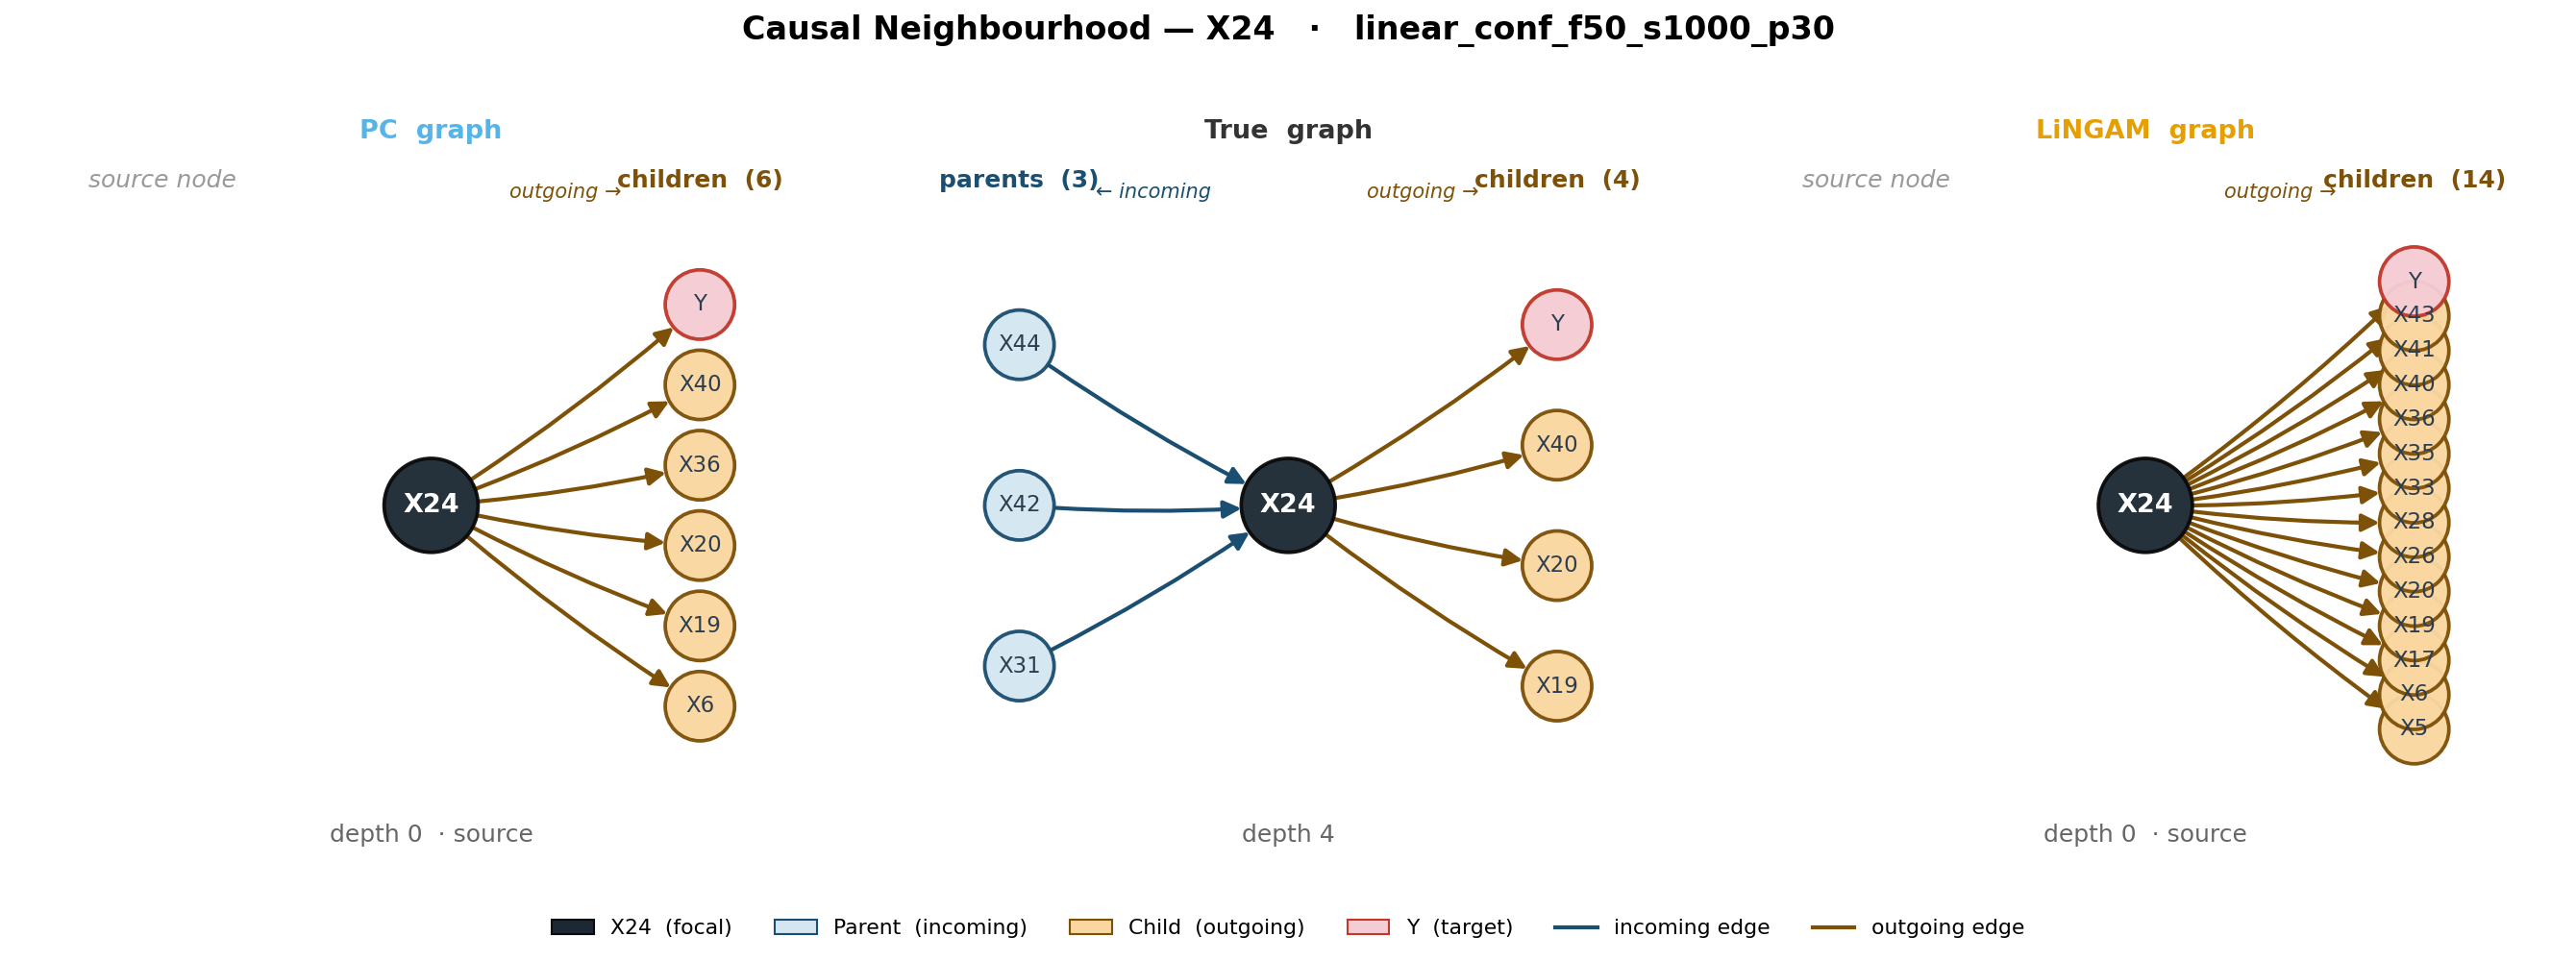
\includegraphics[width=\columnwidth]{figures/dag_neighborhood_X24_linear_conf_f50_s1000_p30.png}
  \caption{\textbf{Causal neighbourhood of X24 (Synthetic).} Both PC and LiNGAM strip
  true parents and add spurious children (6 and 14 out-edges respectively, 0 in-edges),
  converting a mid-graph node into an apparent root source. Blue = incoming, amber = outgoing.}
  \label{fig:dag_X24}
\end{figure}

\begin{figure}[H]
  \centering
  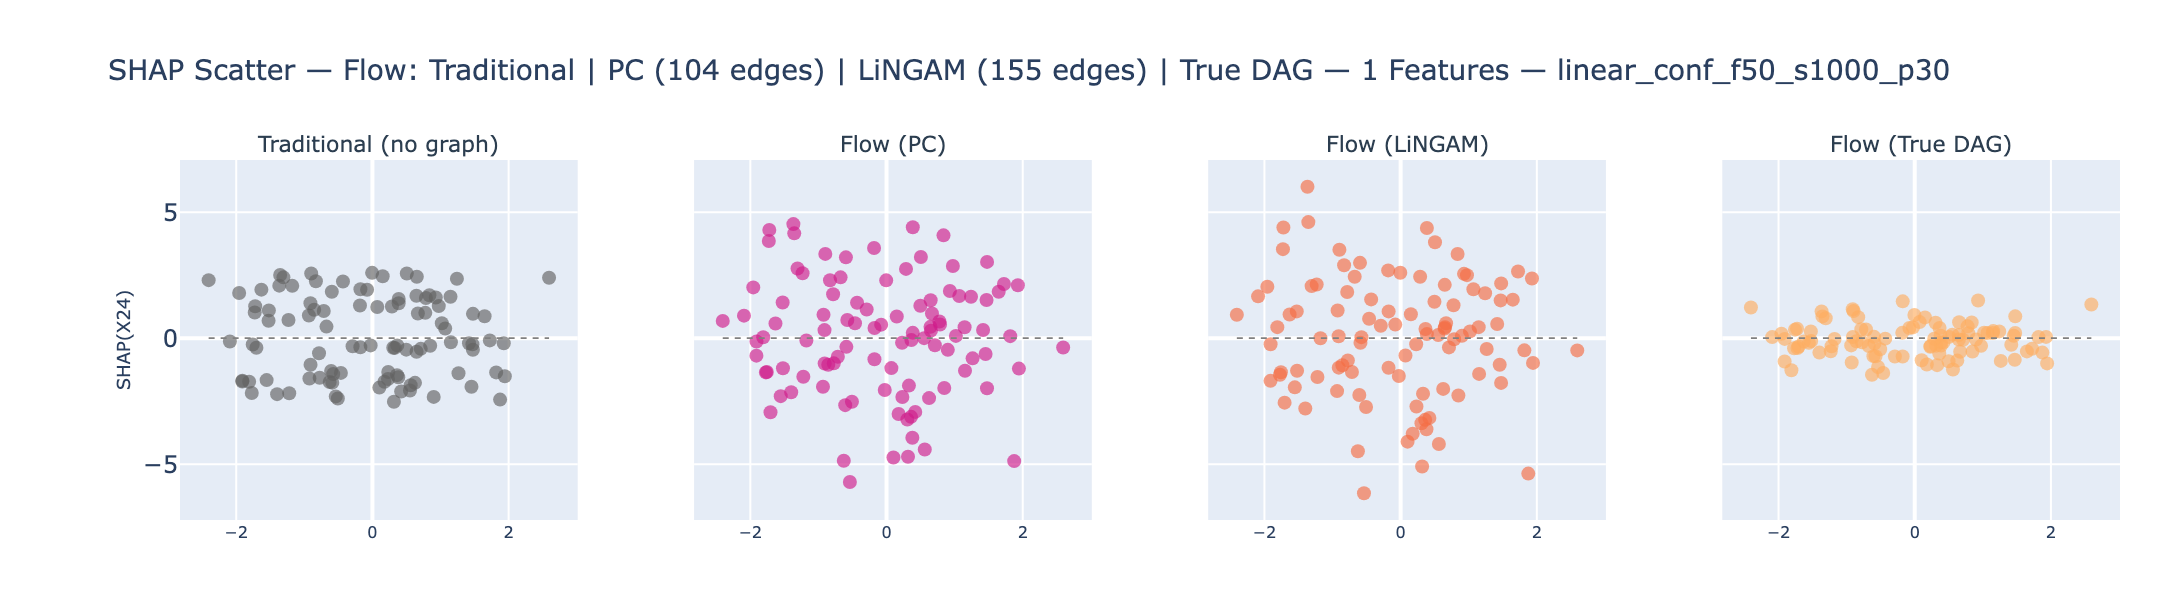
\includegraphics[width=\columnwidth]{figures/shap_scatter_flow_X24_linear_conf_f50_s1000_p30.png}
  \caption{\textbf{Shapley Flow SHAP scatter for X24 (Synthetic).} Traditional shows a
  stable attribution pattern; both discovered-graph columns diverge substantially from
  the True-DAG oracle---the instance-level signature of out-degree inflation
  ($\Delta M_{\text{base}} = 32.5\%$ of $\hat{\sigma}$).}
  \label{fig:shap_X24}
\end{figure}

The same mechanism appears on Sachs through protein pka, a near-root source (1 incoming,
6 outgoing edges in the consensus DAG). LiNGAM preserves this structure accurately,
keeping pka as a near-pure root (ASV $\Delta M_{\text{oracle}} = 6.4\%$ of $\hat{\sigma}$).
PC reverses several of its outgoing edges into a 3-in/3-out configuration, and that
mis-orientation raises pka's ASV $\Delta M_{\text{oracle}}$ to 25.0\%
(Figure~\ref{fig:dag_pka}). A high $\Delta M_{\text{base}}$ (17.3\% of $\hat{\sigma}$)
combined with a large $\Delta M_{\text{disc}}$ forms the two-signal alarm: pka's
discovered connections are both influential and contested across algorithms.

\begin{figure}[H]
  \centering
  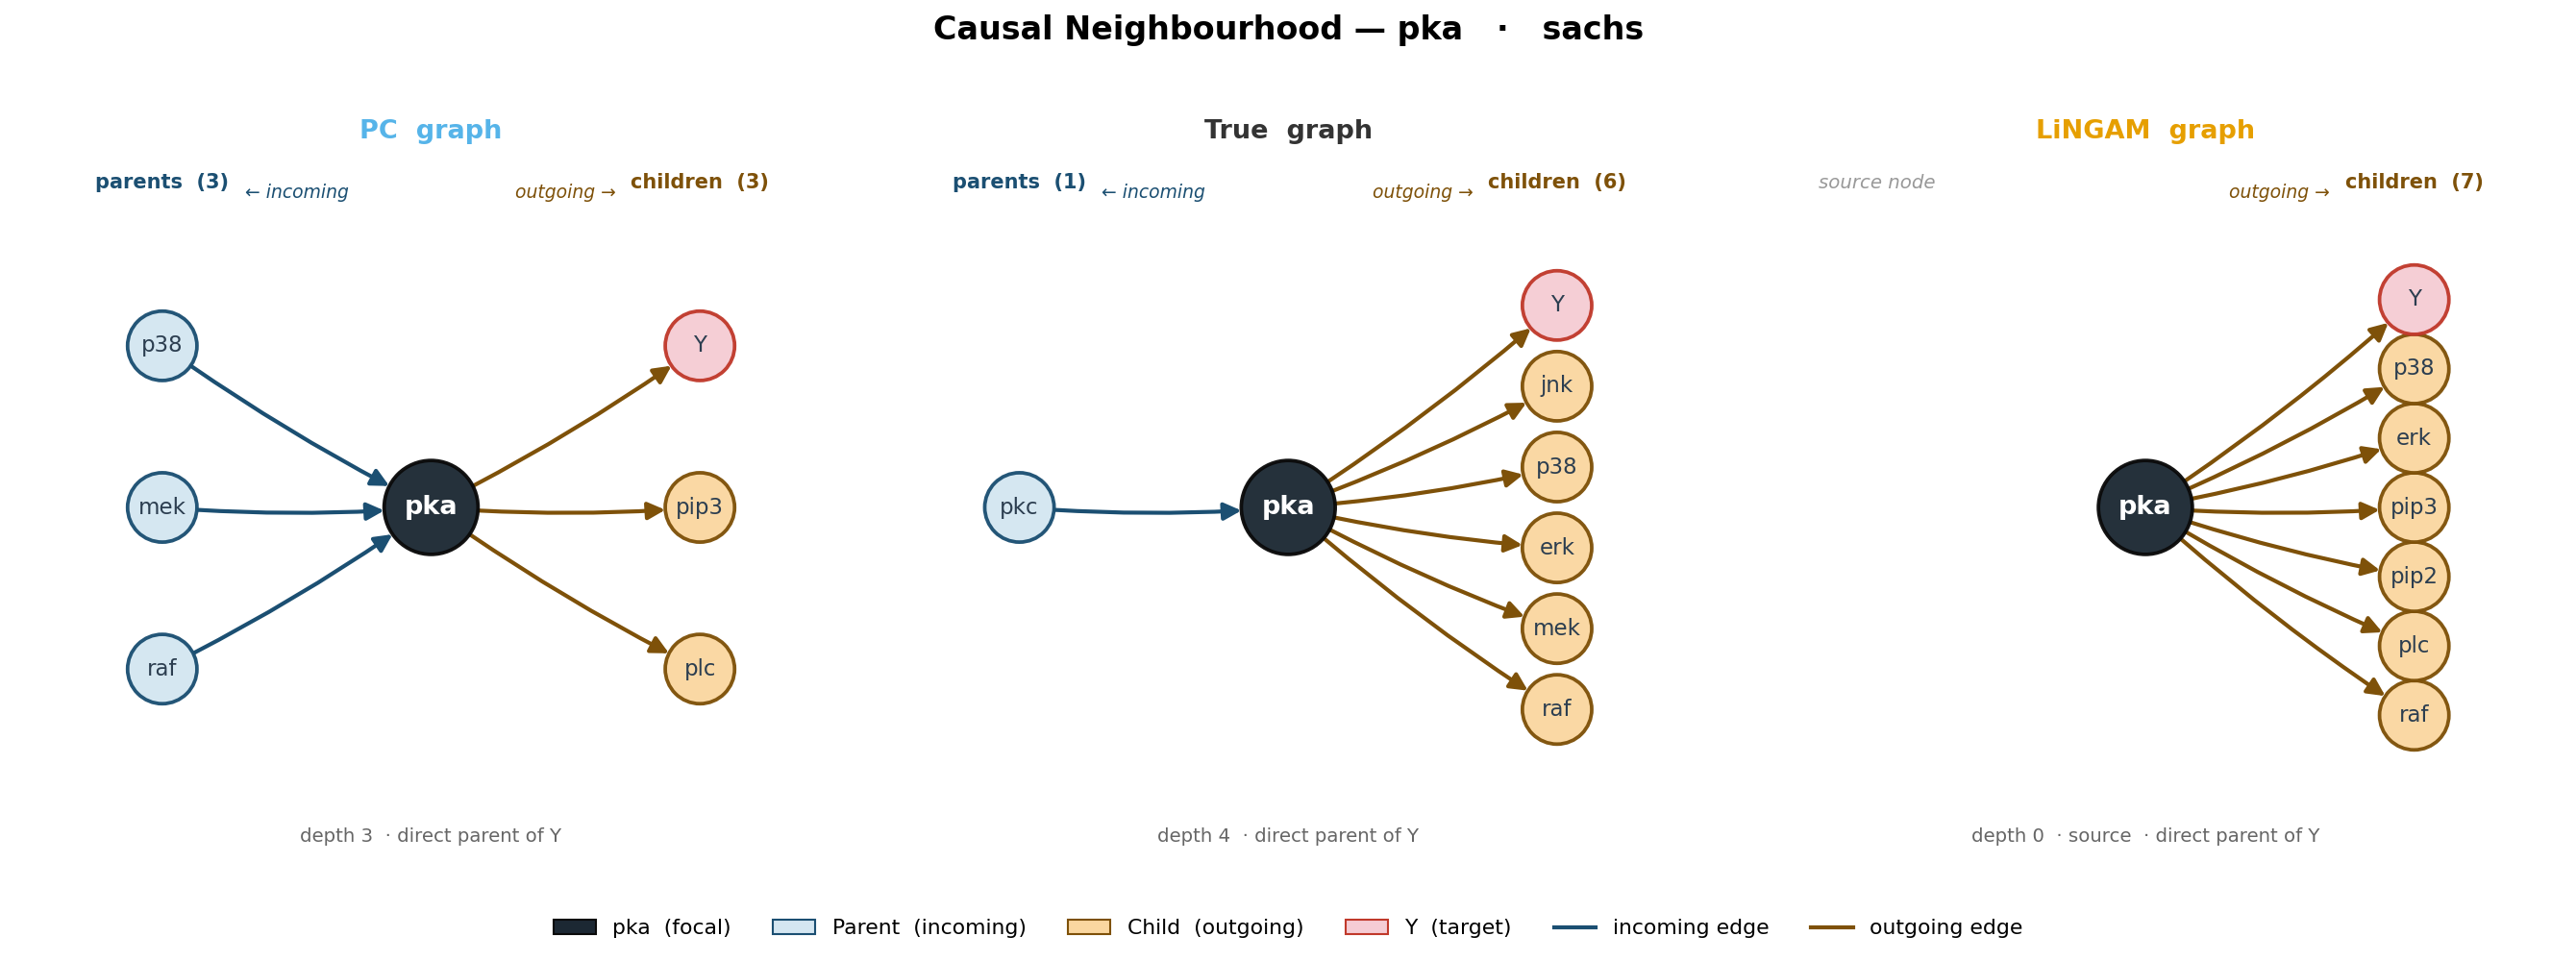
\includegraphics[width=\columnwidth]{figures/dag_neighborhood_pka_sachs.png}
  \caption{\textbf{Causal neighbourhood of pka (Sachs).} PC gives pka 3 incoming and
  3 outgoing edges, reversing several true outgoing links. LiNGAM keeps it a near-root
  with 7 outgoing and 0 incoming edges, much closer to the consensus structure.}
  \label{fig:dag_pka}
\end{figure}

\subsubsection{Directed Edge Inversion and Causal Credit Transfer}

A single edge orientation error by one discovery algorithm can produce a sharply
divergent attribution. In the True DAG the edge runs $X_{21} \to X_{47}$: X21 is a
causal ancestor of X47, which is a dominant direct parent of $Y$. LiNGAM recovers
this orientation correctly; PC reverses it to $X_{47} \to X_{21}$, placing X47 upstream
of X21 (Figure~\ref{fig:dag_X21}).

Under LiNGAM, both CSV and Flow correctly treat X21 as an upstream node, assigning
indirect credit for its causal influence through X47. Under PC the reversed edge injects
X47 into X21's interventional parent set (CSV) and routes edge credit from X47 toward
X21 (Flow), suppressing X47's attribution and inflating X21's. The SHAP scatters
(Figure~\ref{fig:shap_X47_X21}) confirm this: both CSV+LiNGAM and Flow+LiNGAM track
the True-DAG oracle closely, while the PC variants diverge on both features.
Feature-level $\Delta M_{\text{disc}}$ for CSV reaches 29.8\% of $\hat{\sigma}$ on
X47---the two-signal alarm indicating that a real edge's \emph{orientation}, not its
existence, must be resolved before using any structure-aware Shapley method.

\begin{figure}[H]
  \centering
  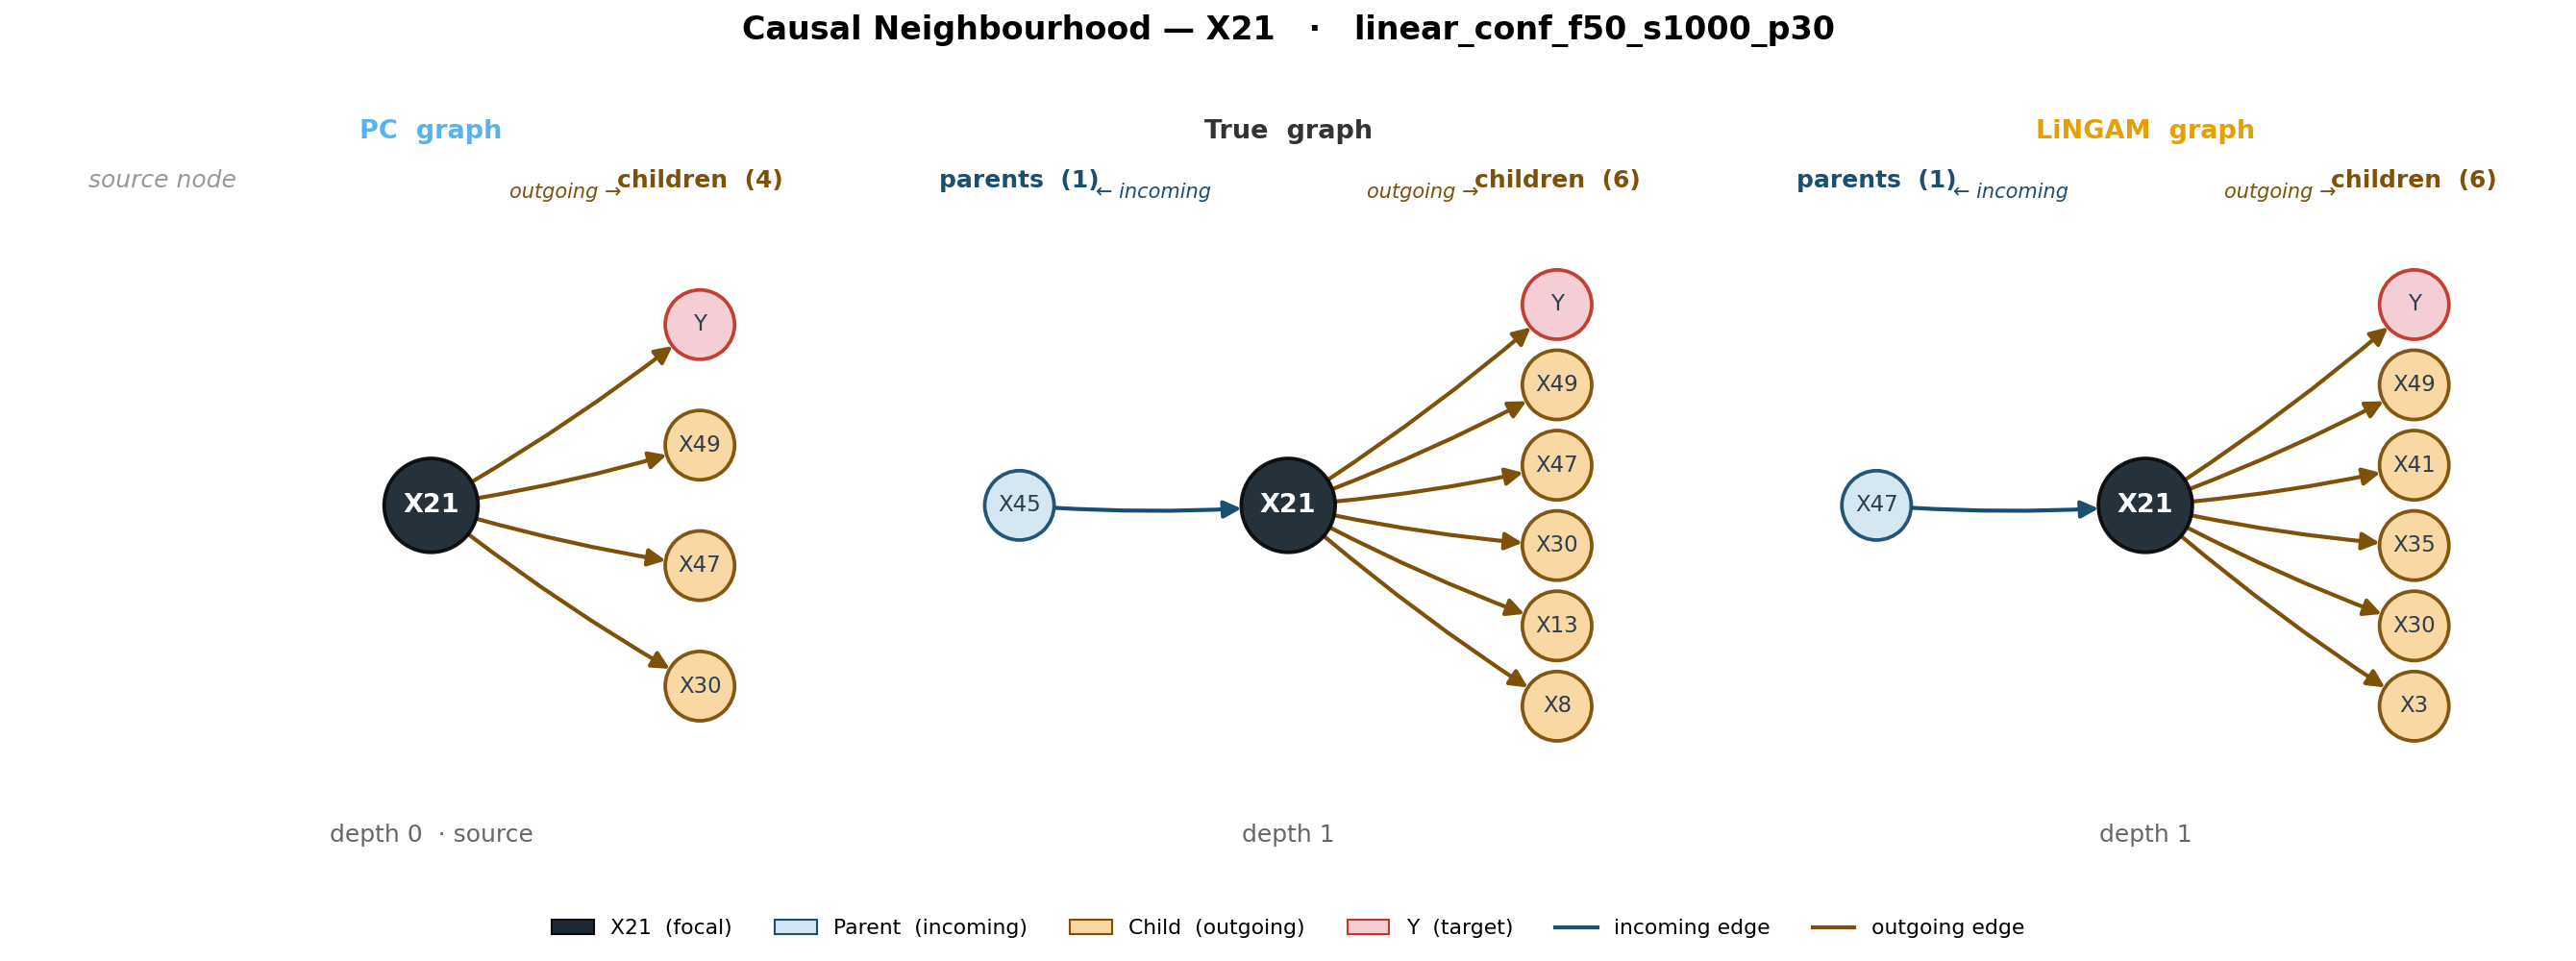
\includegraphics[width=0.85\columnwidth]{figures/dag_neighborhood_X21_linear_conf_f50_s1000_p30.png}
  \caption{\textbf{Causal neighbourhood of X21 (Synthetic).} In the True DAG and under
  LiNGAM the edge runs $X_{21} \to X_{47}$. PC reverses it to $X_{47} \to X_{21}$,
  misdirecting attribution credit in both CSV and Flow.}
  \label{fig:dag_X21}
\end{figure}

\begin{figure}[H]
  \centering
  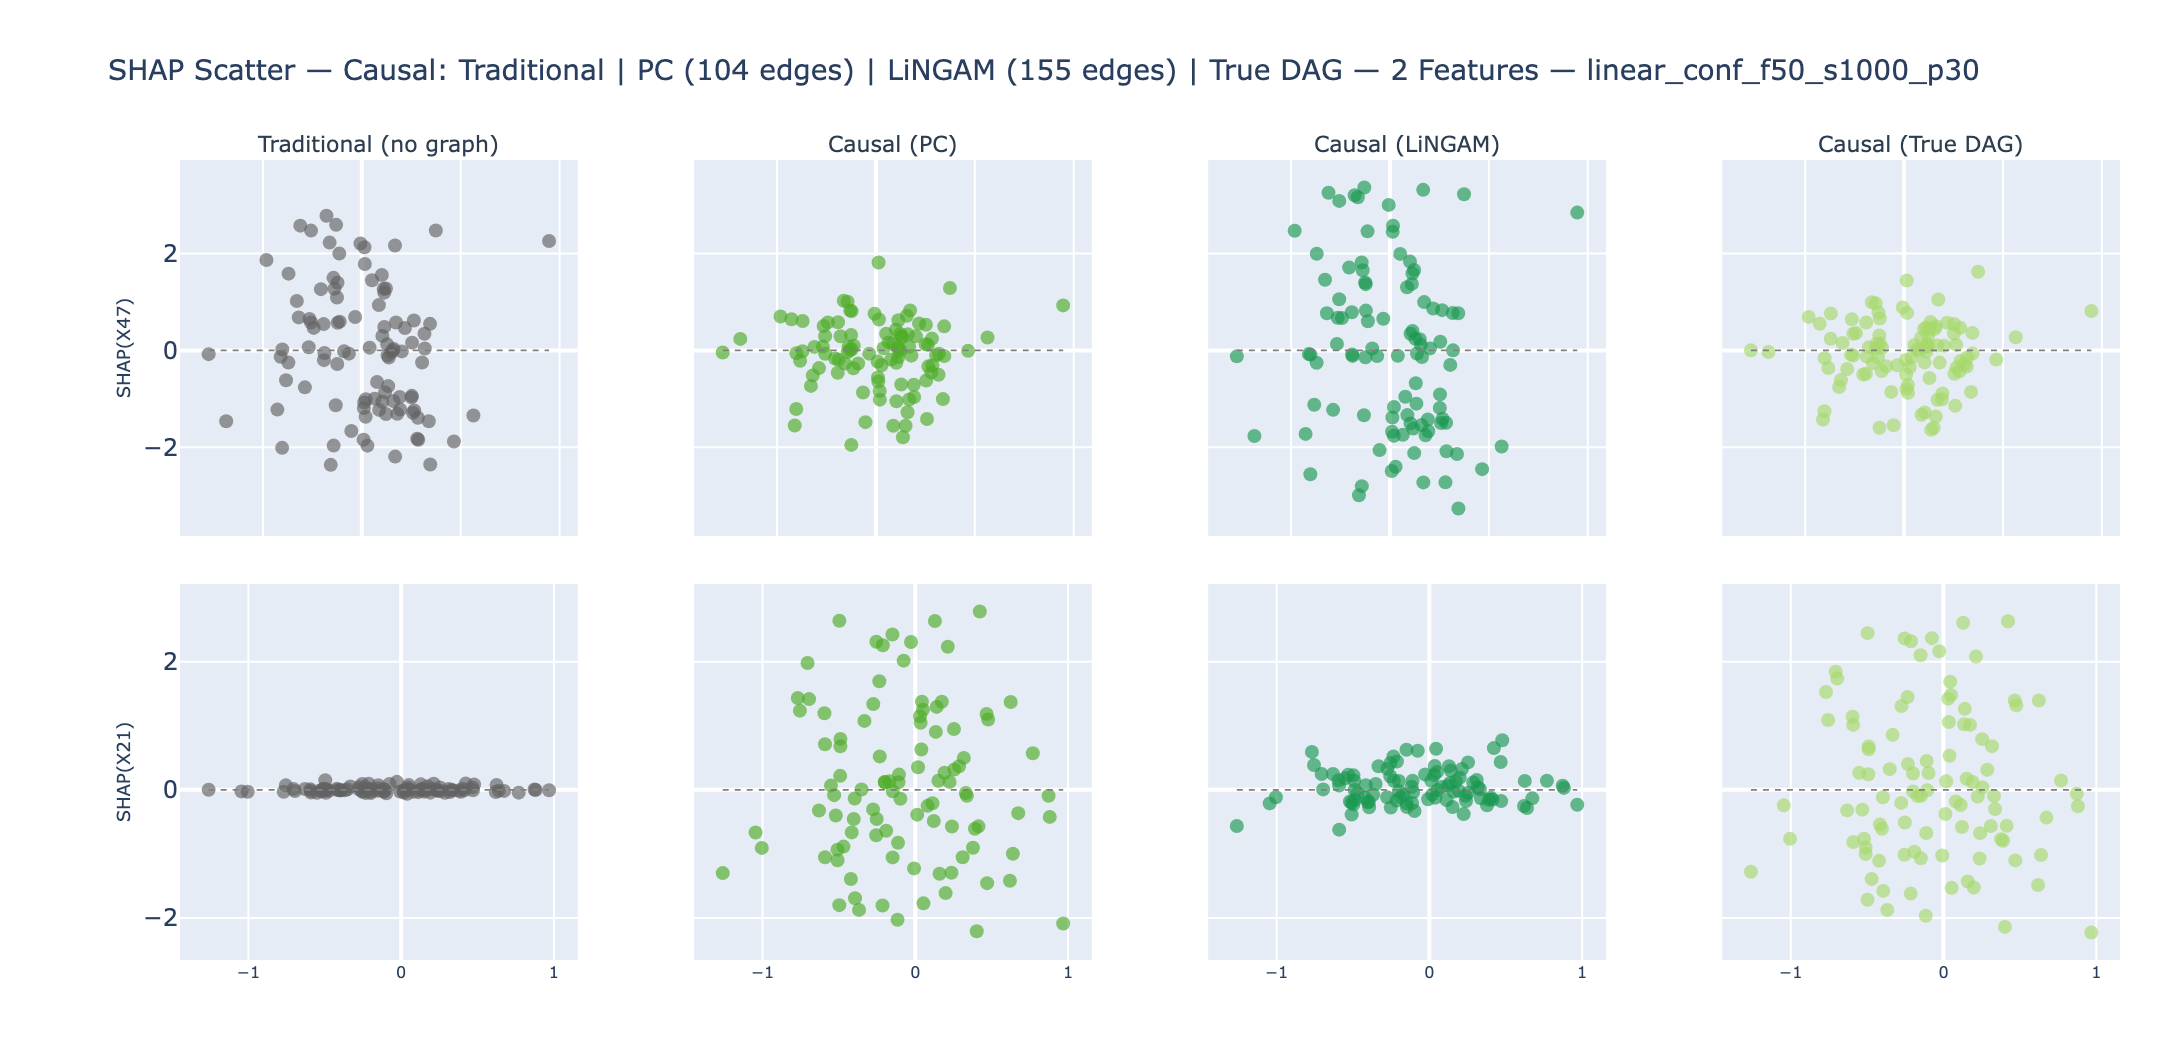
\includegraphics[width=\columnwidth]{figures/shap_scatter_causal_X47_X21_linear_conf_f50_s1000_p30.png}
  \vspace{2pt}
  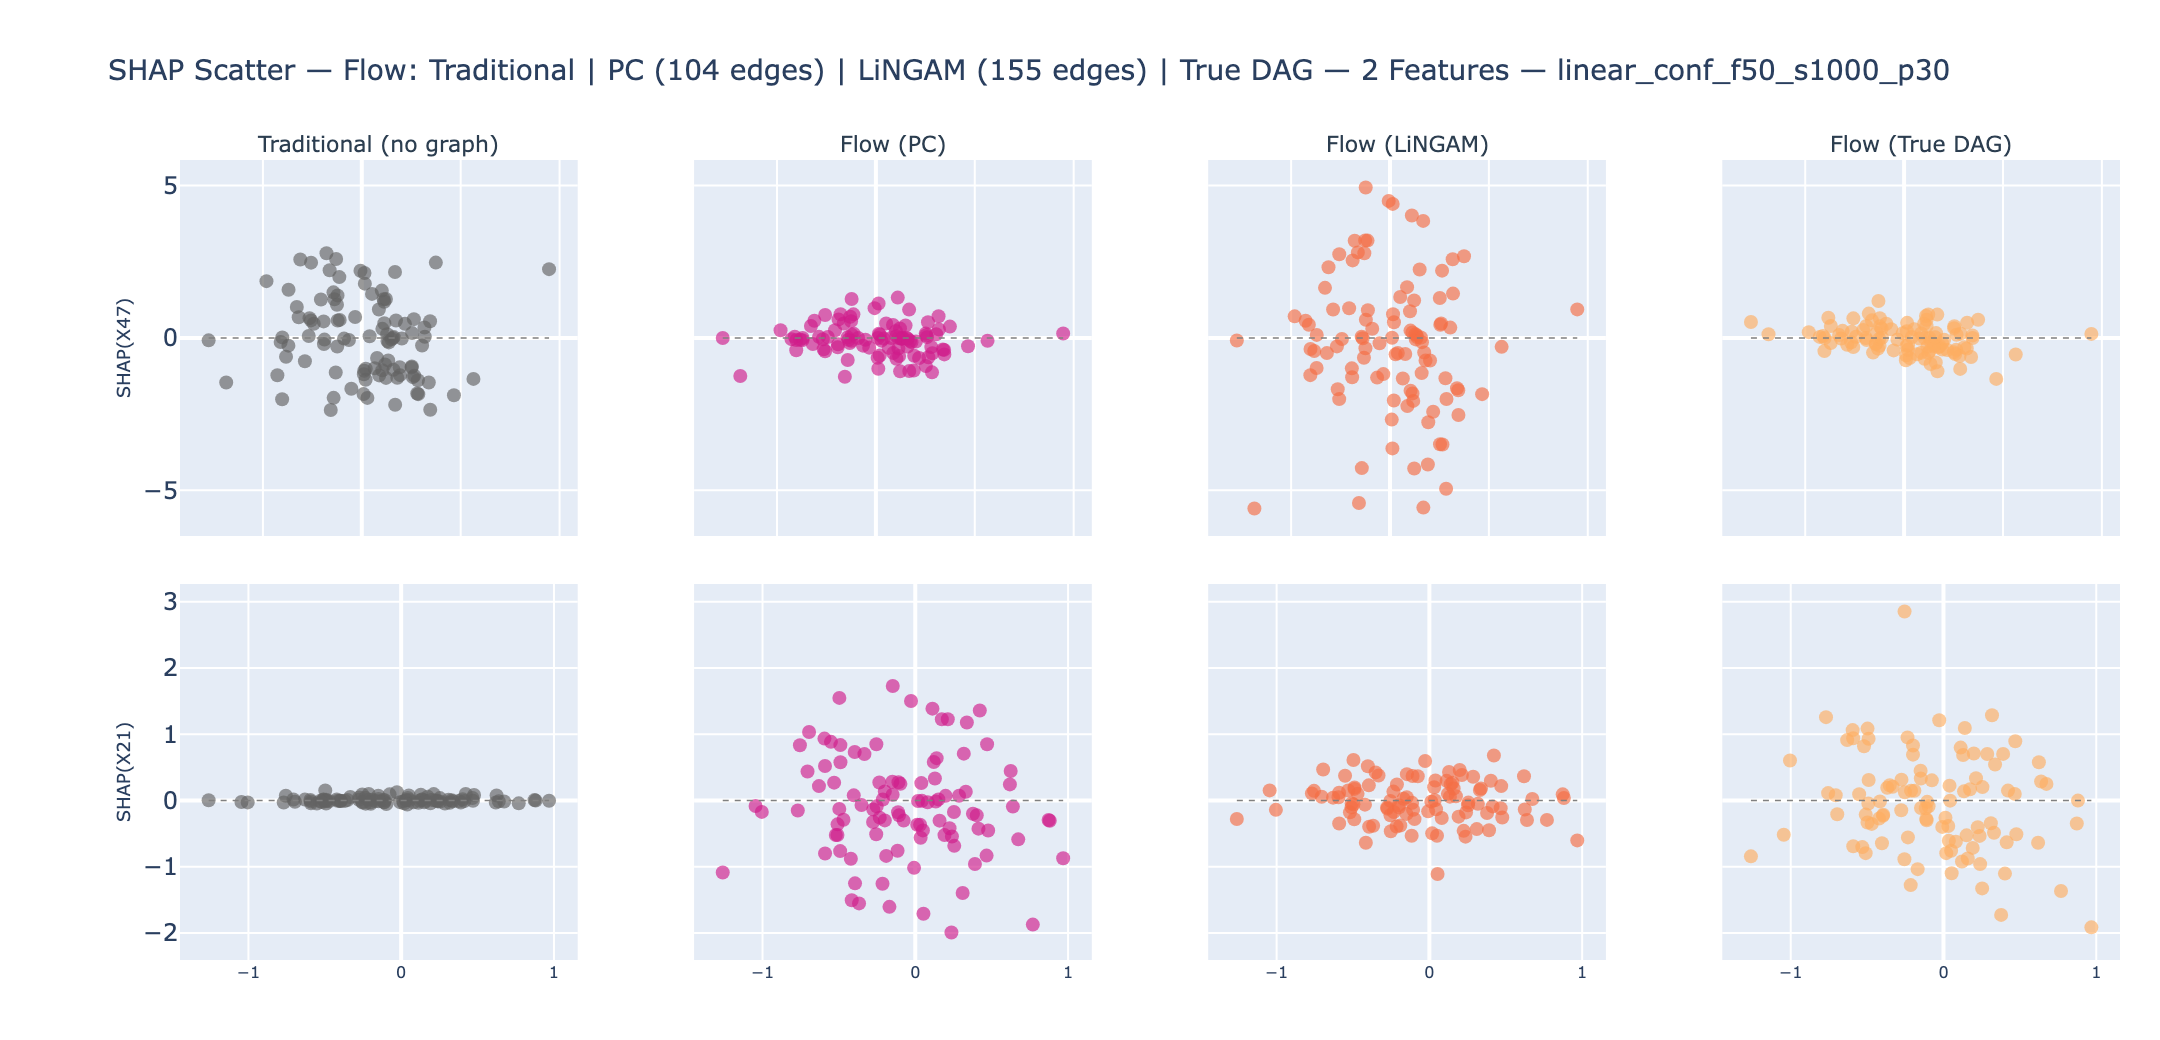
\includegraphics[width=\columnwidth]{figures/shap_scatter_flow_X47_X21_linear_conf_f50_s1000_p30.png}
  \caption{\textbf{SHAP scatter for X21 and X47 (Synthetic).} \textit{Top} (Causal
  Shapley): under LiNGAM both features track the oracle; under PC, X47 is suppressed
  and X21 acquires inflated credit. \textit{Bottom} (Shapley Flow): the same
  orientation-driven credit transfer appears; Flow+LiNGAM and Flow+True agree closely
  while Flow+PC diverges on both features.}
  \label{fig:shap_X47_X21}
\end{figure}

\subsubsection{Confounded Subordination and Boundary Isolation}

Synthetic feature X6 is a true intermediate node with 3 parents and 4 children.
LiNGAM inflates its in-degree to 8 with spurious incoming links; under CSV these false
parents generate an overly constrained post-interventional distribution, yielding a
feature-level $\Delta M_{\text{oracle}} = 28.1\%$ of $\hat{\sigma}$---among the highest
in the synthetic confounded track (Figure~\ref{fig:dag_X6}). The SHAP scatter
(Figure~\ref{fig:shap_X6}) shows the LiNGAM column diverging sharply from both the
Traditional baseline and the True-DAG oracle while PC stays close---a direct consequence
of LiNGAM inflating X6's in-degree and contaminating its interventional conditioning
set. This makes the precision and recall of the discovery step a direct, visible factor
in CSV's reliability.

\begin{figure}[H]
  \centering
  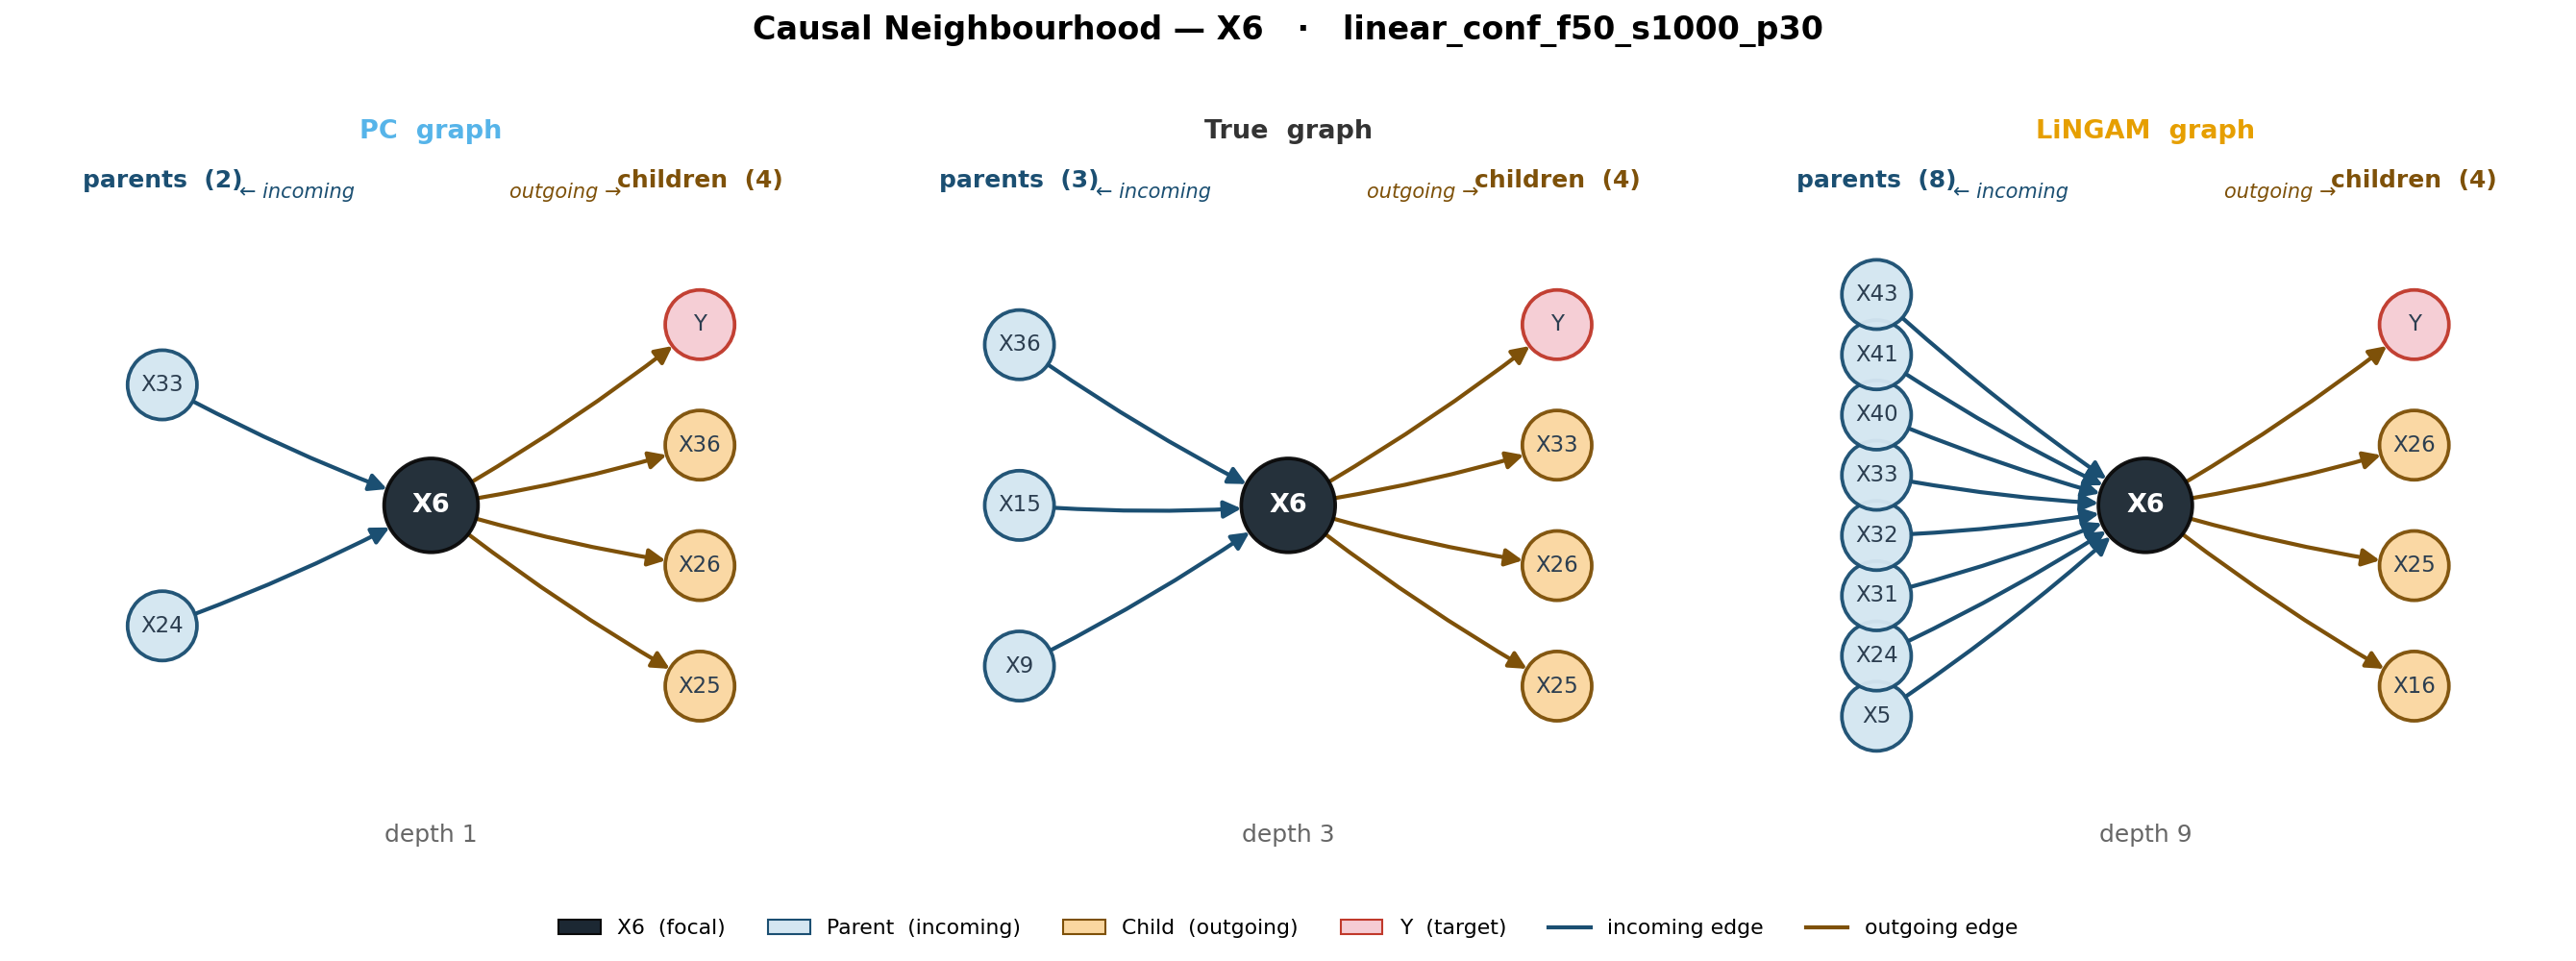
\includegraphics[width=0.85\columnwidth]{figures/dag_neighborhood_X6_linear_conf_f50_s1000_p30.png}
  \caption{\textbf{Causal neighbourhood of X6 (Synthetic).} X6 has 3 incoming and 4
  outgoing edges in the True DAG. LiNGAM inflates its in-degree to 8, contaminating
  its interventional conditioning set under CSV.}
  \label{fig:dag_X6}
\end{figure}

\begin{figure}[H]
  \centering
  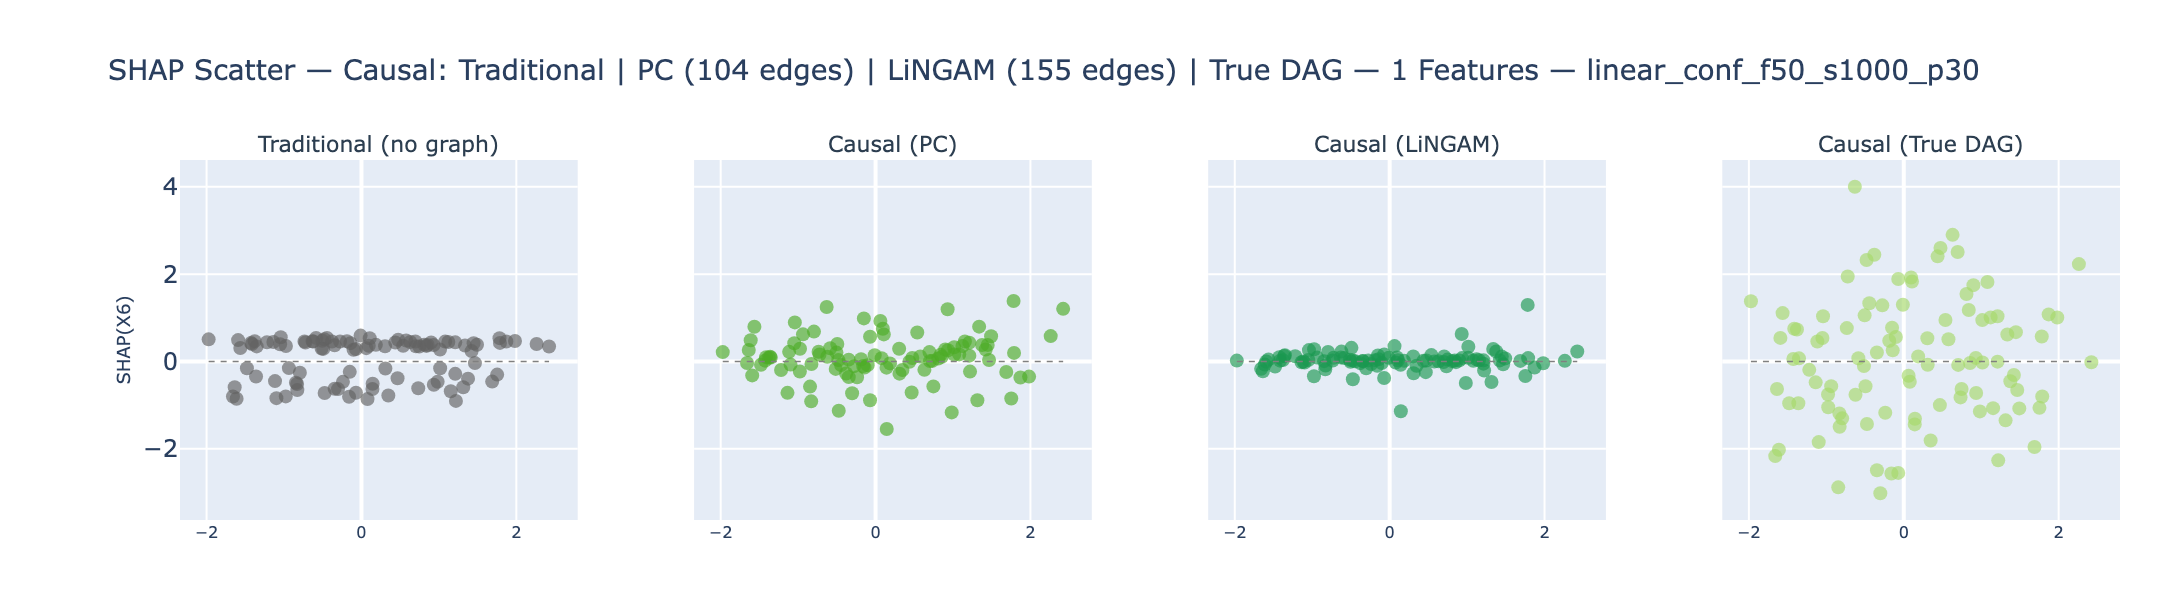
\includegraphics[width=\columnwidth]{figures/shap_scatter_causal_X6_linear_conf_f50_s1000_p30.png}
  \caption{\textbf{Causal Shapley SHAP scatter for X6 (Synthetic).} The LiNGAM column
  diverges sharply from both the Traditional baseline and the True-DAG oracle; PC stays
  close---a direct consequence of LiNGAM's in-degree inflation from 3 to 8.}
  \label{fig:shap_X6}
\end{figure}

On Sachs, protein erk is a downstream node receiving inputs from pka and mek in the
consensus DAG. PC removes its parent links and isolates it as a root source with several
outgoing edges (Figure~\ref{fig:dag_erk}), giving erk a disproportionately large Flow
attribution ($\Delta M_{\text{oracle}} = 49.2\%$ of $\hat{\sigma}$ for Flow+PC, the
largest single deviation in the real-data experiment). The SHAP scatter
(Figure~\ref{fig:shap_erk}) shows all three graph-aware variants producing materially
different attribution patterns: Flow+PC inflates erk by treating it as a source;
Flow+LiNGAM produces a distinct distortion; only Flow+True DAG tracks the correct
downstream credit distribution. Across all three metrics---$\Delta M_{\text{base}}$,
$\Delta M_{\text{oracle}}$, and $\Delta M_{\text{disc}}$---erk is simultaneously far
from the graph-free baseline, far from the oracle, and far from itself under a different
algorithm. This triple divergence is the framework's strongest warning signal.

\begin{figure}[H]
  \centering
  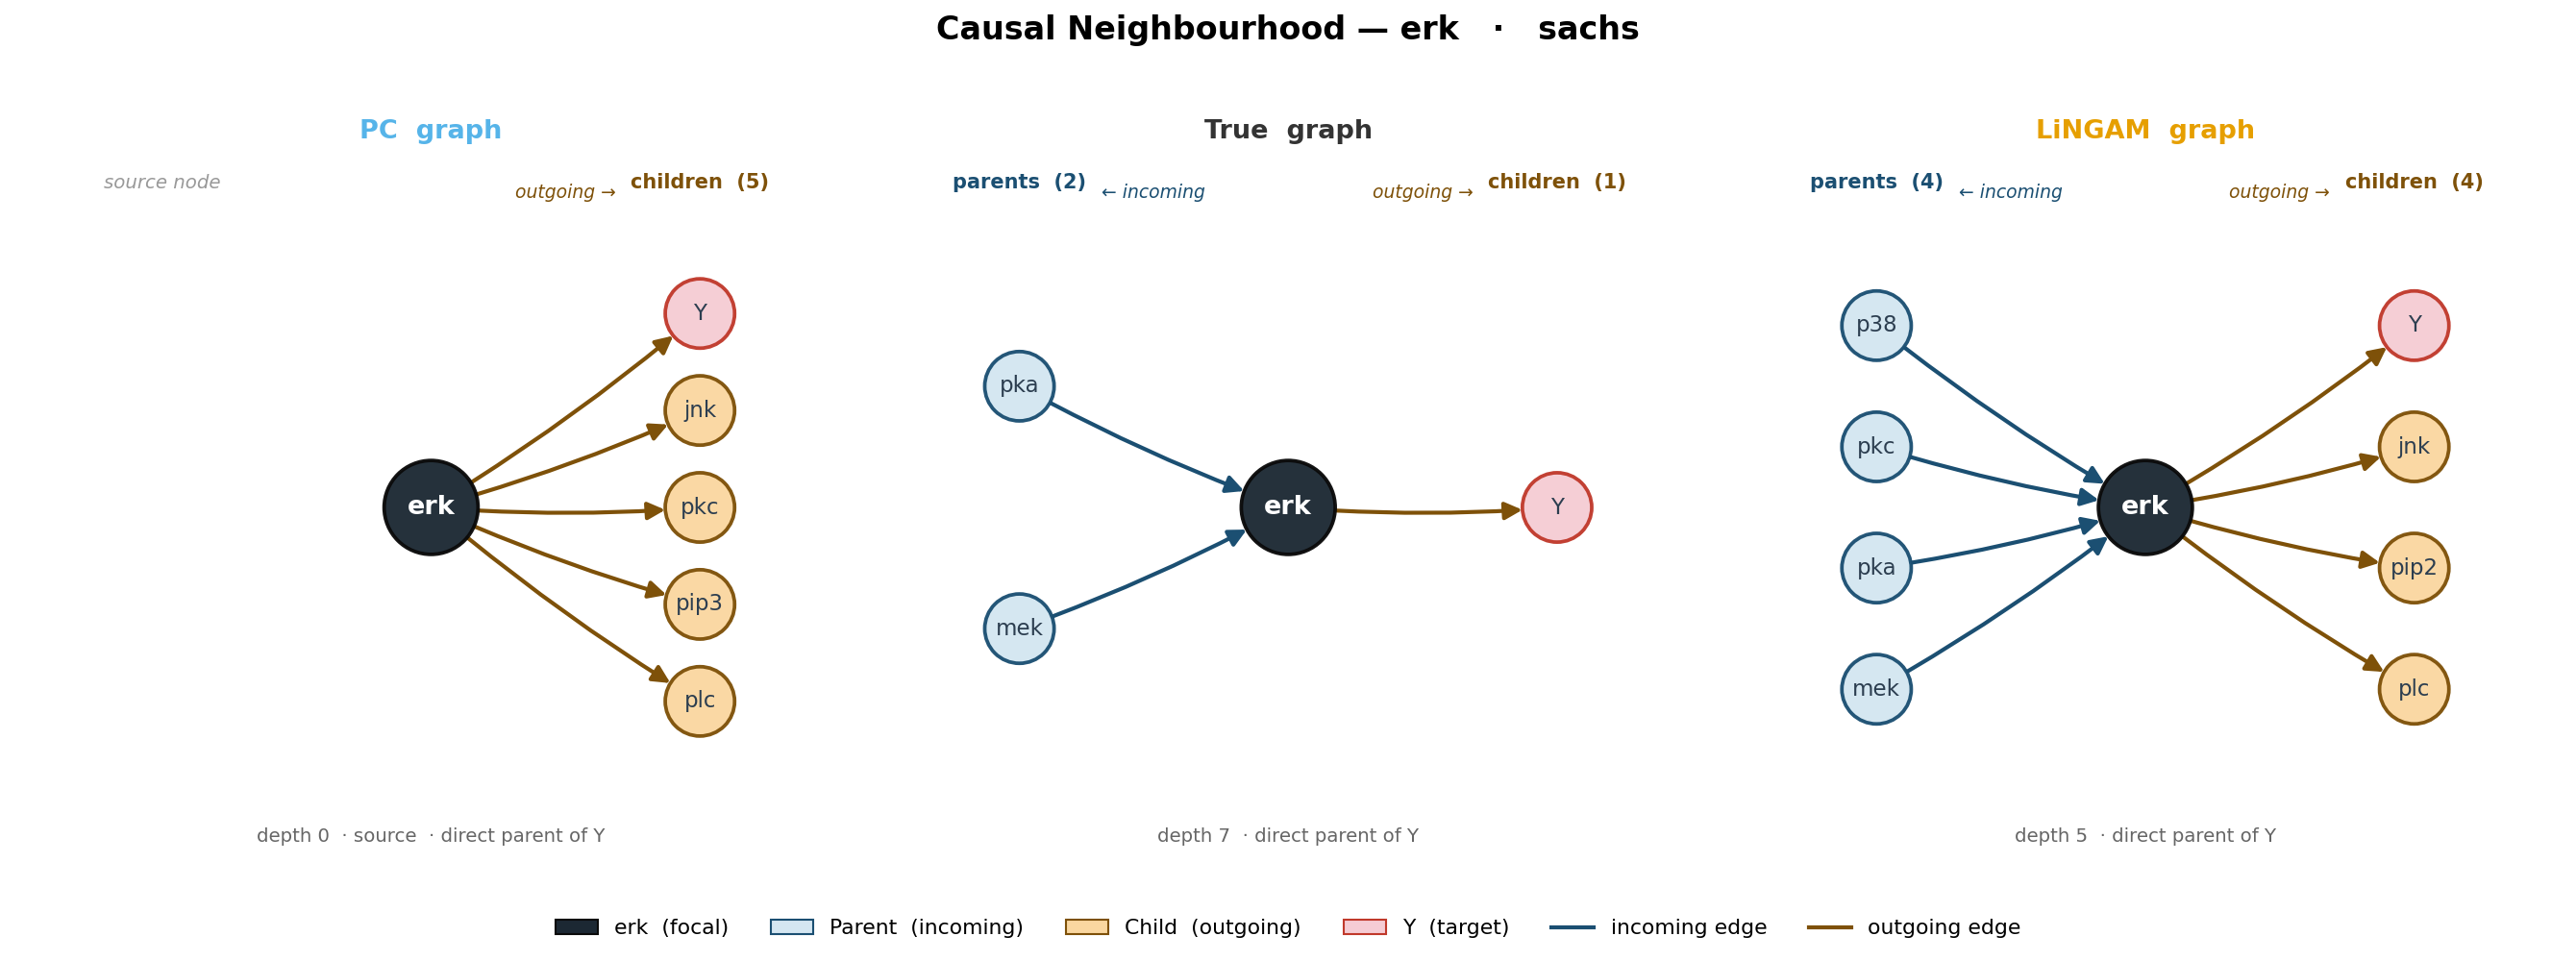
\includegraphics[width=\columnwidth]{figures/dag_neighborhood_erk_sachs.png}
  \caption{\textbf{Causal neighbourhood of erk (Sachs).} PC removes its true parent
  links (pka, mek) and isolates erk as a boundary source---driving Flow+PC's
  $\Delta M_{\text{oracle}} = 49.2\%$ of $\hat{\sigma}$.}
  \label{fig:dag_erk}
\end{figure}

\begin{figure}[H]
  \centering
  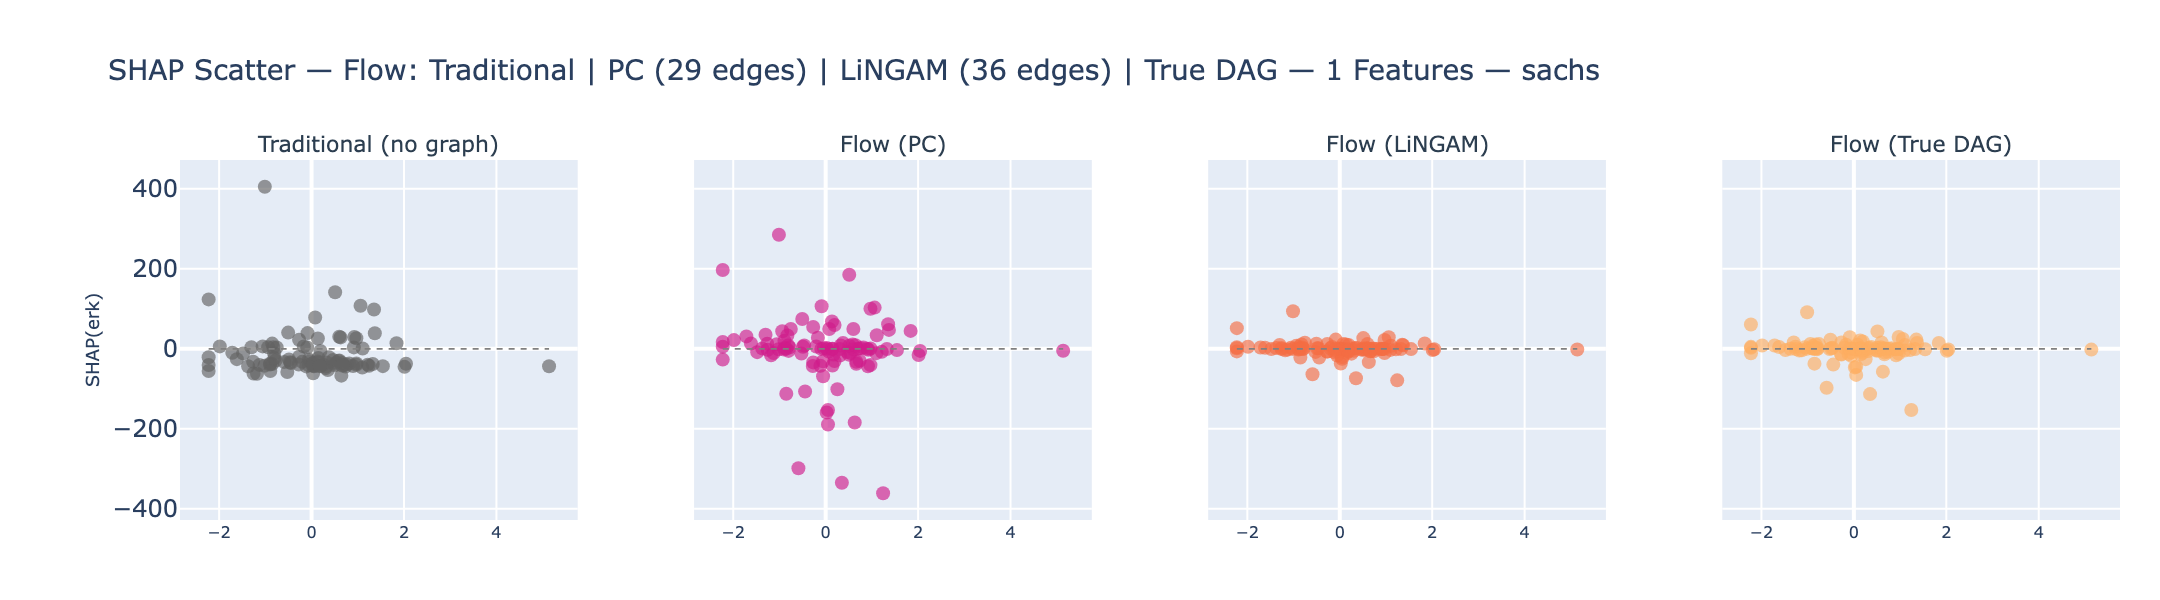
\includegraphics[width=\columnwidth]{figures/shap_scatter_flow_erk_sachs.png}
  \caption{\textbf{Shapley Flow SHAP scatter for erk (Sachs).} All three graph-aware
  variants diverge from each other and from Traditional. Flow+PC inflates erk's
  attributions by treating it as an isolated source node; only Flow+True DAG tracks the
  correct downstream credit distribution.}
  \label{fig:shap_erk}
\end{figure}

%% ============================================================
\section{Conclusion}
\label{sec:conclusion}
%% ============================================================

\subsection{Summary of Findings}

This work built an experimental pipeline to measure what happens to feature attributions
when you plug an automatically discovered causal graph into a structure-aware Shapley
method. The three Shapley methods fall into completely different sensitivity regimes. ASV
is stable under graph errors, specially in sparse high-dimensional datasets: on the
50-feature synthetic data, swapping the True DAG for a discovered graph moves ASV's
attributions by less than 1.1\% of $\hat{\sigma}$ and flips fewer than 7\% of attribution
signs. This stability comes from ASV's core logic---it only restricts the permutation
space, leaving the observational value function untouched, so most topological orderings
remain compatible across the true and discovered graphs. CSV and Flow's core logic instead
injects the graph into the conditioning set or into the players themselves, so every false
edge contaminates an attribution directly. Even though, the experimental pipeline allows
spotting features that have structural divergences shifting the explanations badly, which
would allow practitioners to spot improvement points even in ASV before committing to
any structure-aware attribution.

The two discovery algorithms swap rankings across datasets (PC better on synthetic,
LiNGAM better on Sachs) and neither reaches high accuracy on either. The real question
is not which algorithm is generally better, but how much the chosen Shapley method
amplifies the errors that algorithm makes. A method sensitive to graph quality, like CSV
or Flow, inherits the weaknesses of whatever discovery algorithm is used; ASV absorbs
them. This shifts the practical decision: rather than finding the best discovery
algorithm, it is more productive to first check how sensitive the Shapley method is to
graph errors on the specific data at hand, and only invest in graph improvement where
sensitivity is high.

The evaluation metrics reveal things you cannot see by looking at attributions alone.
A high $\Delta M_{\text{base}}$ on a node flags that the injected graph is doing a lot
of work there (X24: 32.5\%, X6: 28.1\%, pka: 17.3\%). When $\Delta M_{\text{base}}$
and $\Delta M_{\text{disc}}$ are both high on the same node, the graph structure for
that feature is both influential and contested: the two-signal alarm. erk on Sachs adds
a third signal ($\Delta M_{\text{oracle}}$ also high), the clearest warning the framework
can emit.

\subsection{Practical Recommendations}

The most important contribution is the evaluation framework itself. Before this work, a
practitioner adding a discovered graph to a Shapley computation had no systematic way
to assess what that decision would cost in attribution quality. The six metrics at both
dataset and feature level give a structured vocabulary for this assessment. In most
real-world scenarios only the base and disc metrics are available; those are the ones
the framework is really built around. The practical ordering is clear:

\begin{itemize}[nosep]
  \item \textbf{ASV is the recommended default.} It delivers oracle-level alignment with
  minimal deviation from the Traditional baseline, works well even with poor discovery
  results (Sachs PC: F1 = 0.167), and adds no computational cost above standard Monte
  Carlo SHAP.
  \item \textbf{CSV and Flow are useful only when graph quality is high}---when domain
  experts have validated the structure, or when the cross-discovery stability metrics
  confirm the graph is stable. CSV+LiNGAM on confounded synthetic produces
  $D_{\text{oracle}} = 37.5\%$ and $D_{\text{disc}} = 37.9\%$: attributions differ in
  sign from the oracle more than a third of the time and disagree with themselves across
  graph sources at the same rate. That level of instability makes explanations
  inconsistent across audit runs and difficult to defend in practice.
\end{itemize}

\subsection{Limitations and Future Work}

The analysis covers a single synthetic functional form (linear confounded) and one real
dataset; nonlinear and mixed functional forms, different graph densities, and larger
sample sizes remain to be tested. All Shapley computations use $T = 100$ Monte Carlo
samples. Future work should extend to nonlinear Shapley variants, explore ensemble
approaches averaging attributions across multiple discovered graphs to reduce
cross-discovery instability, and investigate whether active learning strategies could
use the feature-level $\Delta M_{\text{disc}}$ signal to guide targeted graph refinement
starting from the nodes the framework identifies as most contested.

%% ============================================================
\newpage
\bibliography{references}

%% ============================================================
%% Appendix — uncounted pages
%% ============================================================
\onecolumn
\appendix

\section{Detailed Results Tables}
\label{app:tables}

\subsection{Baseline Deviation (vs.\ Traditional Shapley)}

\begin{table}[H]
  \centering
  \caption{\textbf{Baseline Deviation -- Linear-Conf Synthetic Dataset.}}
  \label{tab:baseline_synth}
  \begin{tabular}{llrr}
    \toprule
    \textbf{Method} & \textbf{Graph} & $D_{\text{base}}$ & $\Delta M_{\text{base}}$ \\
    \midrule
    Asymmetric & PC     & 5.08\%  & 0.68\% \\
    Asymmetric & LiNGAM & 5.76\%  & 0.86\% \\
    Causal     & PC     & 35.30\% & 6.39\% \\
    Causal     & LiNGAM & 33.92\% & 5.84\% \\
    Flow       & PC     & 36.58\% & 6.62\% \\
    Flow       & LiNGAM & 37.68\% & 6.61\% \\
    \bottomrule
  \end{tabular}
\end{table}

\begin{table}[H]
  \centering
  \caption{\textbf{Baseline Deviation -- Sachs Cell Signaling Dataset.}}
  \label{tab:baseline_sachs}
  \begin{tabular}{llrr}
    \toprule
    \textbf{Method} & \textbf{Graph} & $D_{\text{base}}$ & $\Delta M_{\text{base}}$ \\
    \midrule
    Asymmetric & PC     & 16.80\% & 5.08\%  \\
    Asymmetric & LiNGAM & 17.00\% & 4.41\%  \\
    Causal     & PC     & 31.30\% & 7.83\%  \\
    Causal     & LiNGAM & 33.10\% & 9.31\%  \\
    Flow       & PC     & 40.20\% & 12.68\% \\
    Flow       & LiNGAM & 41.50\% & 14.17\% \\
    \bottomrule
  \end{tabular}
\end{table}

\subsection{Oracle Alignment (vs.\ True / Consensus DAG)}

\begin{table}[H]
  \centering
  \caption{\textbf{Oracle Alignment -- Linear-Conf Synthetic Dataset.}
  $D_{\text{oracle}}$ and $\Delta M_{\text{oracle}}$ in \% of $\hat{\sigma}$.}
  \label{tab:oracle_synth}
  \begin{tabular}{llrr}
    \toprule
    \textbf{Method} & \textbf{Graph} & $D_{\text{oracle}}$ & $\Delta M_{\text{oracle}}$ \\
    \midrule
    Asymmetric & PC     & 5.88\%  & 1.02\% \\
    Asymmetric & LiNGAM & 6.30\%  & 0.79\% \\
    Causal     & PC     & 31.60\% & 5.32\% \\
    Causal     & LiNGAM & 37.46\% & 7.57\% \\
    Flow       & PC     & 42.26\% & 7.34\% \\
    Flow       & LiNGAM & 44.91\% & 8.06\% \\
    \bottomrule
  \end{tabular}
\end{table}

\begin{table}[H]
  \centering
  \caption{\textbf{Oracle Alignment -- Sachs Cell Signaling Dataset (oracle = consensus
  DAG).} $D_{\text{oracle}}$ and $\Delta M_{\text{oracle}}$ in \% of $\hat{\sigma}$.}
  \label{tab:oracle_sachs}
  \begin{tabular}{llrr}
    \toprule
    \textbf{Method} & \textbf{Graph} & $D_{\text{oracle}}$ & $\Delta M_{\text{oracle}}$ \\
    \midrule
    Asymmetric & PC     & 24.26\% & 9.16\%  \\
    Asymmetric & LiNGAM & 23.40\% & 2.84\%  \\
    Causal     & PC     & 36.30\% & 9.01\%  \\
    Causal     & LiNGAM & 32.30\% & 8.31\%  \\
    Flow       & PC     & 28.36\% & 15.52\% \\
    Flow       & LiNGAM & 23.81\% & 8.12\%  \\
    \bottomrule
  \end{tabular}
\end{table}

\subsection{Cross-Discovery Sensitivity (PC vs.\ LiNGAM)}

\begin{table}[H]
  \centering
  \caption{\textbf{PC vs.\ LiNGAM Sensitivity -- Linear-Conf Synthetic Dataset.}}
  \label{tab:disc_synth}
  \begin{tabular}{lrr}
    \toprule
    \textbf{Method} & $\Delta M_{\text{disc}}$ & $D_{\text{disc}}$ \\
    \midrule
    Asymmetric & 1.07\%  & 5.93\%  \\
    Causal     & 7.15\%  & 37.94\% \\
    Flow       & 6.06\%  & 13.27\% \\
    \bottomrule
  \end{tabular}
\end{table}

\begin{table}[H]
  \centering
  \caption{\textbf{PC vs.\ LiNGAM Sensitivity -- Sachs Cell Signaling Dataset.}}
  \label{tab:disc_sachs}
  \begin{tabular}{lrr}
    \toprule
    \textbf{Method} & $\Delta M_{\text{disc}}$ & $D_{\text{disc}}$ \\
    \midrule
    Asymmetric & 8.46\%  & 18.60\% \\
    Causal     & 10.11\% & 31.80\% \\
    Flow       & 14.92\% & 21.88\% \\
    \bottomrule
  \end{tabular}
\end{table}

\subsection{Discovery Adjacency Matrices}

\begin{figure}[H]
  \centering
  \begin{subfigure}[t]{0.48\linewidth}
    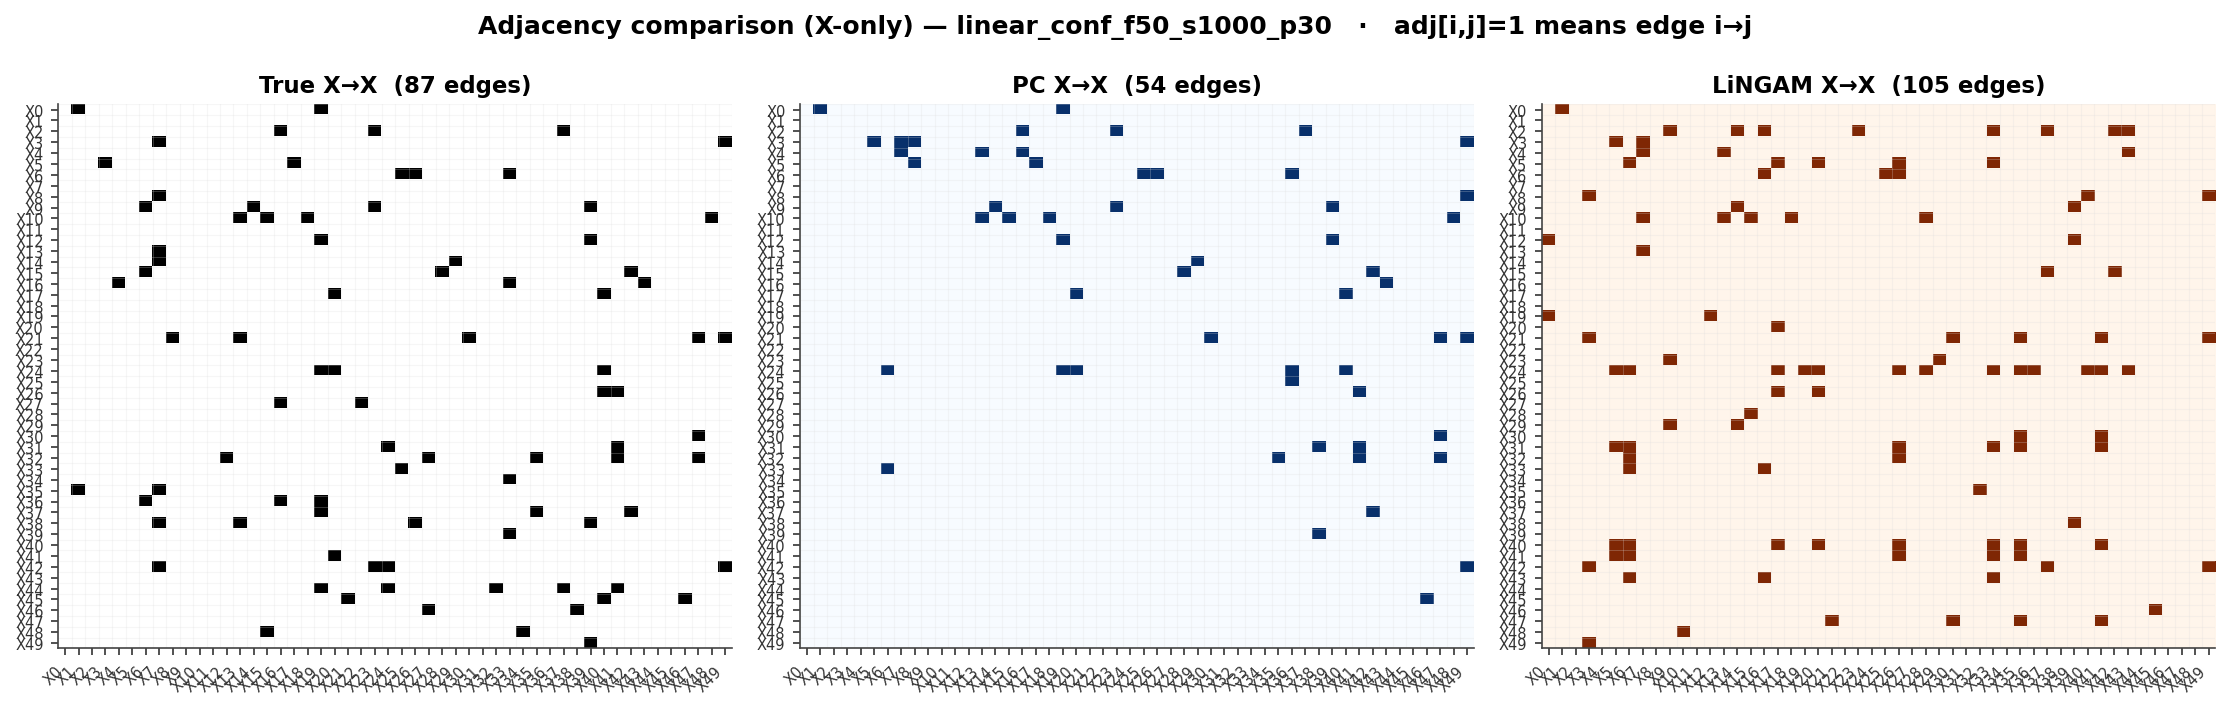
\includegraphics[width=\linewidth]{figures/adjacency_comparison_linear_conf_f50_s1000_p30.png}
    \caption{Synthetic: True DAG (87 edges), PC (54), LiNGAM (105). LiNGAM scatters
    spurious edges across the matrix.}
    \label{fig:adj_synthetic}
  \end{subfigure}
  \hfill
  \begin{subfigure}[t]{0.48\linewidth}
    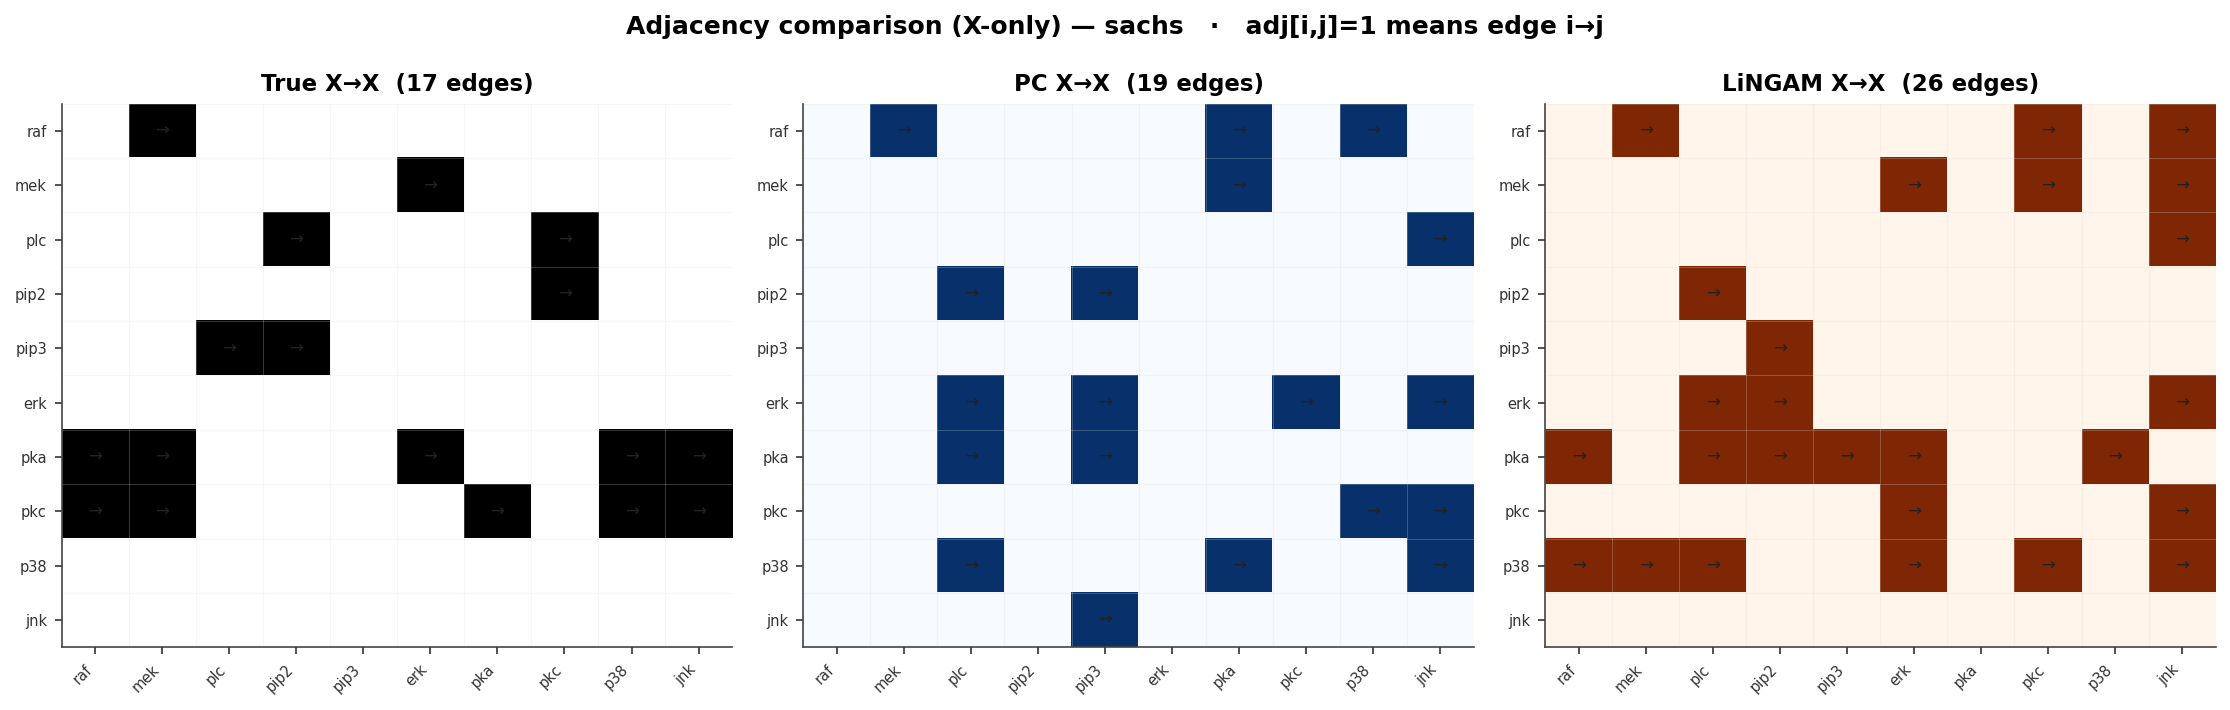
\includegraphics[width=\linewidth]{figures/adjacency_comparison_sachs.png}
    \caption{Sachs: consensus DAG (17 edges), PC (19), LiNGAM (26). Both algorithms
    recover only a fraction of true links.}
    \label{fig:adj_sachs}
  \end{subfigure}
  \caption{\textbf{$X \to X$ adjacency matrices.} $\mathrm{adj}[i,j]=1$ denotes
  $i \to j$. The discovery-quality ordering reverses between datasets.}
  \label{fig:adj_pair}
\end{figure}

%% ============================================================
\subsection{Feature-Level Magnitude Heatmaps ($\Delta M$)}
\label{app:heatmaps_magnitude}

Each heatmap shows $\Delta M^{\mathrm{ref}}_f$ for the top 10 features by mean
divergence. Rows are method-graph combinations; columns are features. Darker cells
indicate larger attribution magnitude shifts. The same top features dominate all three
comparisons.

\begin{figure}[H]
  \centering
  \begin{subfigure}[t]{0.48\linewidth}
    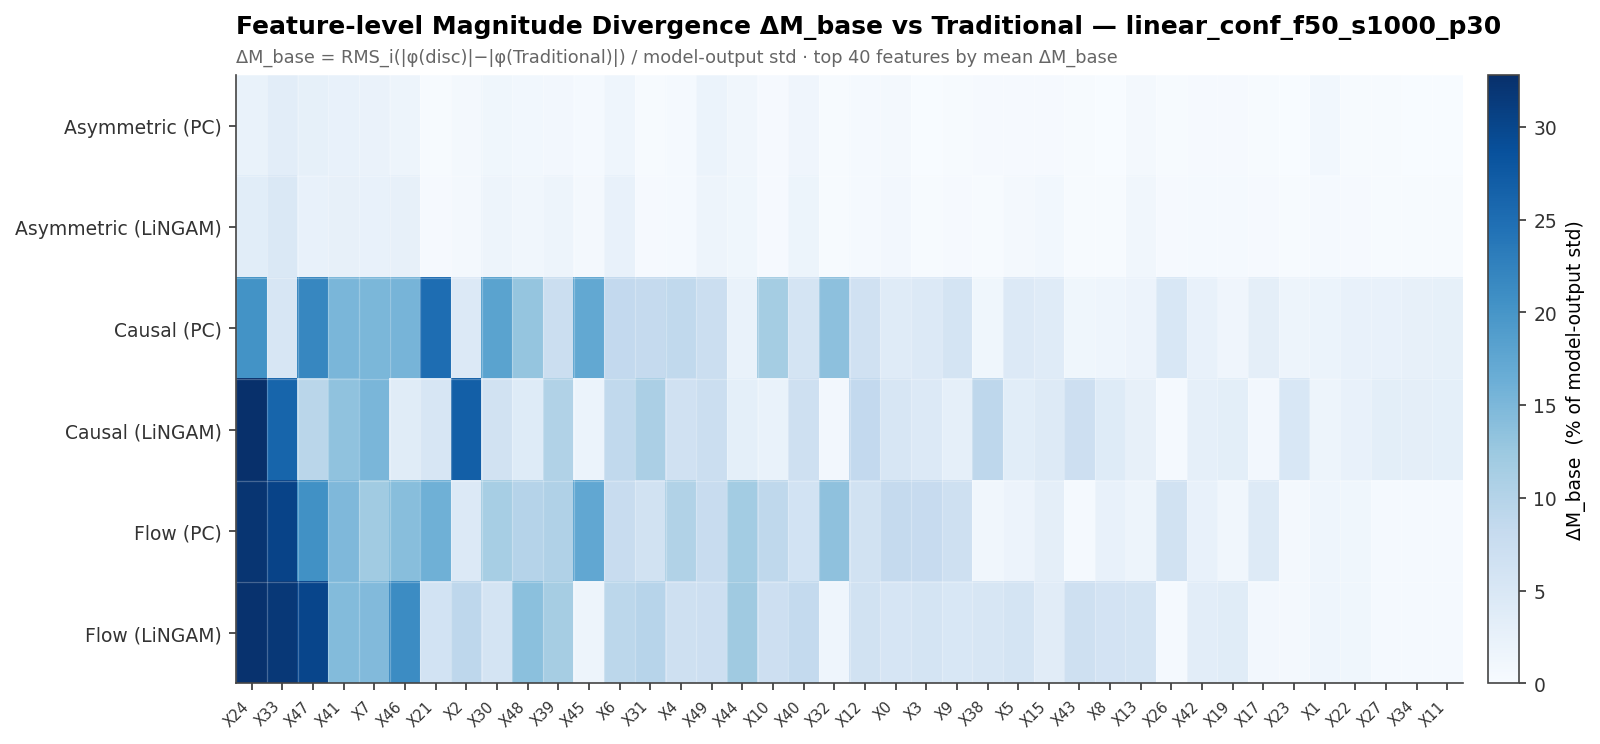
\includegraphics[width=\linewidth]{figures/tga_heatmap_traditional_linear_conf_f50_s1000_p30.png}
    \caption{Synthetic. Asymmetric rows near-zero throughout; Causal and Flow
    concentrate on X24, X33, X47.}
    \label{fig:heatmap_trad_synth}
  \end{subfigure}
  \hfill
  \begin{subfigure}[t]{0.48\linewidth}
    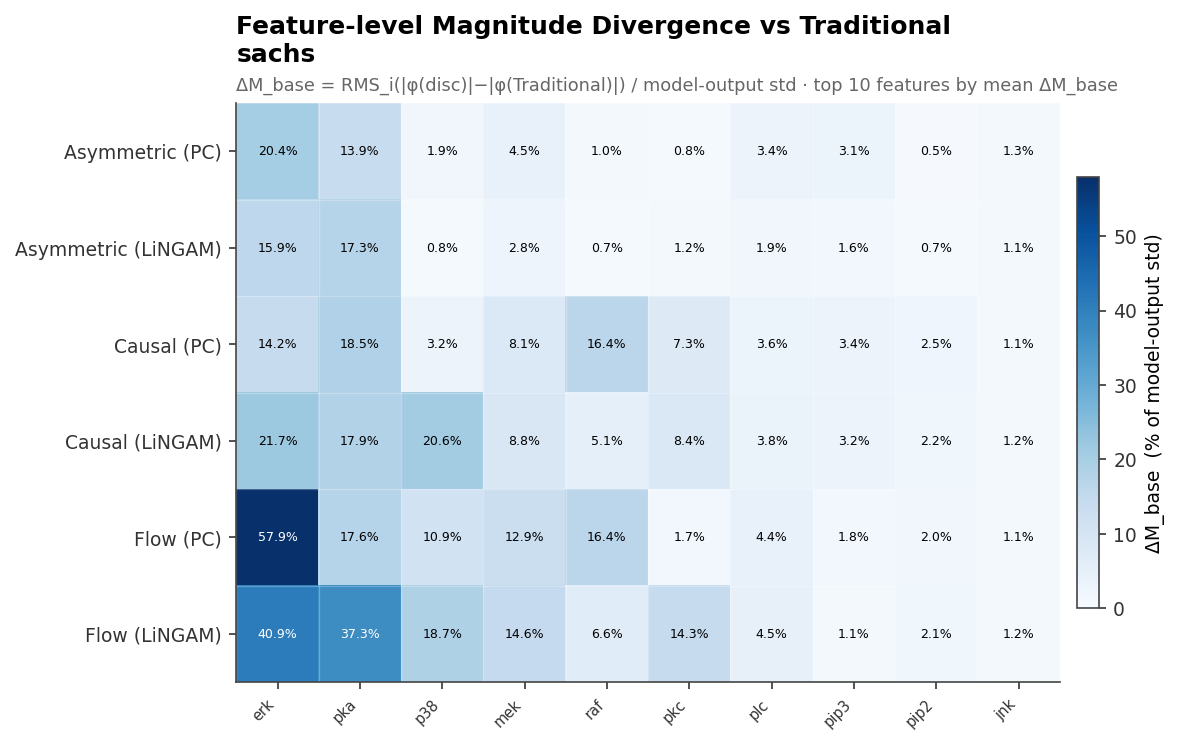
\includegraphics[width=\linewidth]{figures/tga_heatmap_traditional_sachs.png}
    \caption{Sachs. Deviation concentrates on erk and pka; Flow+PC produces
    the largest single shift (erk, 57.9\% of $\hat{\sigma}$).}
    \label{fig:heatmap_trad_sachs}
  \end{subfigure}
  \caption{\textbf{Feature-level $\Delta M_{\text{base}}$ vs.\ Traditional Shapley.}}
  \label{fig:heatmap_trad}
\end{figure}

\begin{figure}[H]
  \centering
  \begin{subfigure}[t]{0.48\linewidth}
    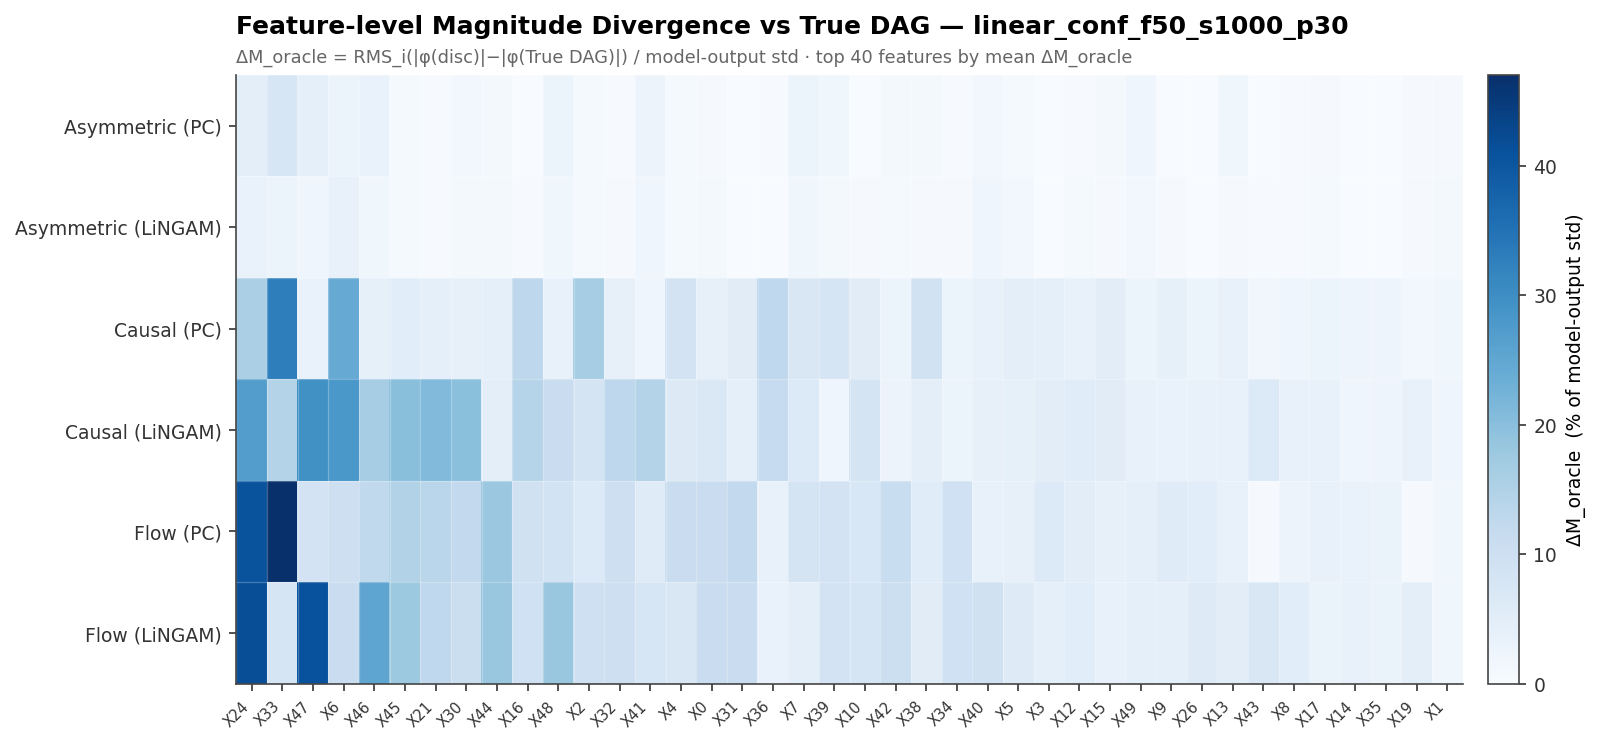
\includegraphics[width=\linewidth]{figures/tga_heatmap_true_linear_conf_f50_s1000_p30.png}
    \caption{Synthetic. Asymmetric rows near-zero; Causal and Flow concentrate
    oracle deviations on X24, X33, X47, X6.}
    \label{fig:heatmap_oracle_synth}
  \end{subfigure}
  \hfill
  \begin{subfigure}[t]{0.48\linewidth}
    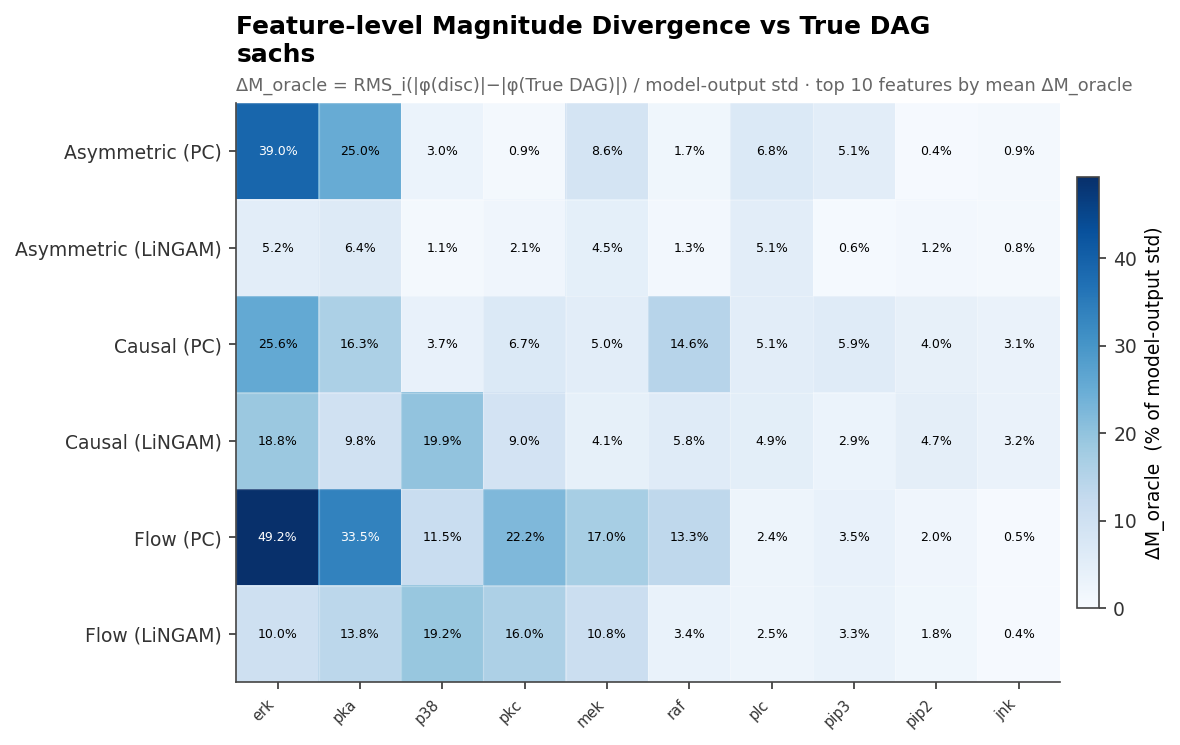
\includegraphics[width=\linewidth]{figures/tga_heatmap_true_sachs.png}
    \caption{Sachs. Flow+PC produces the largest single deviation on erk
    (49.2\% of $\hat{\sigma}$).}
    \label{fig:heatmap_oracle_sachs}
  \end{subfigure}
  \caption{\textbf{Feature-level $\Delta M_{\text{oracle}}$ vs.\ the oracle DAG.}}
  \label{fig:heatmap_oracle}
\end{figure}

\begin{figure}[H]
  \centering
  \begin{subfigure}[t]{0.48\linewidth}
    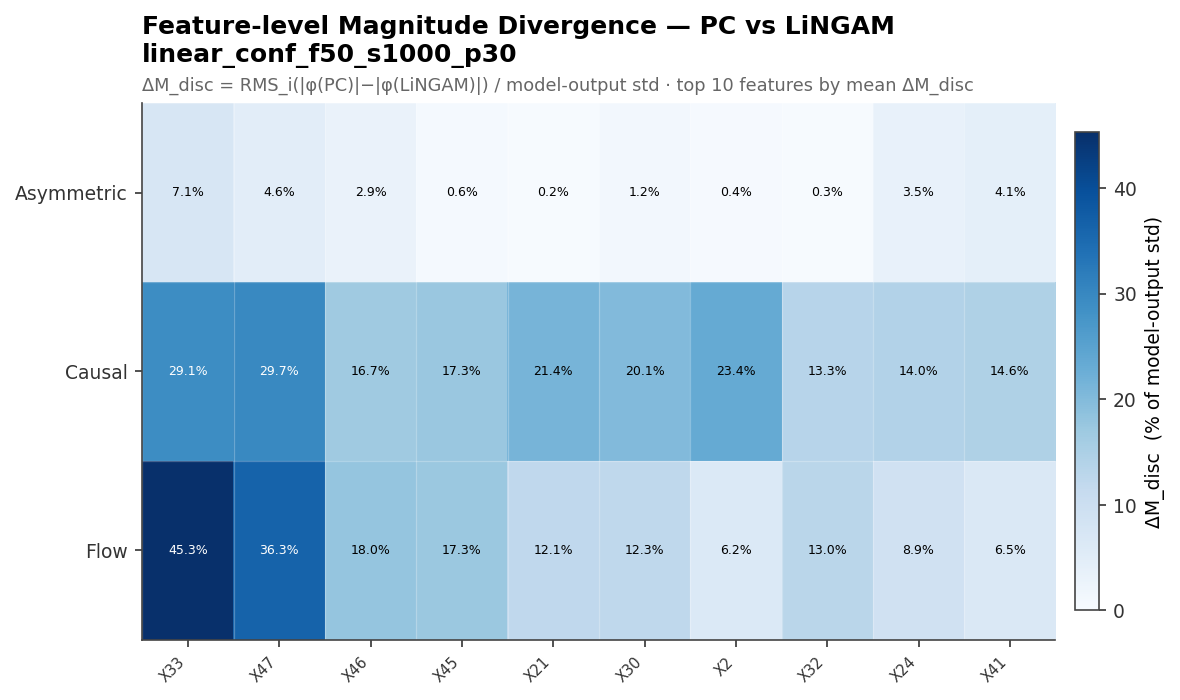
\includegraphics[width=\linewidth]{figures/gss_heatmap_linear_conf_f50_s1000_p30.png}
    \caption{Synthetic. Asymmetric near-zero; Causal and Flow concentrate on X33
    and X47.}
    \label{fig:heatmap_disc_synth}
  \end{subfigure}
  \hfill
  \begin{subfigure}[t]{0.48\linewidth}
    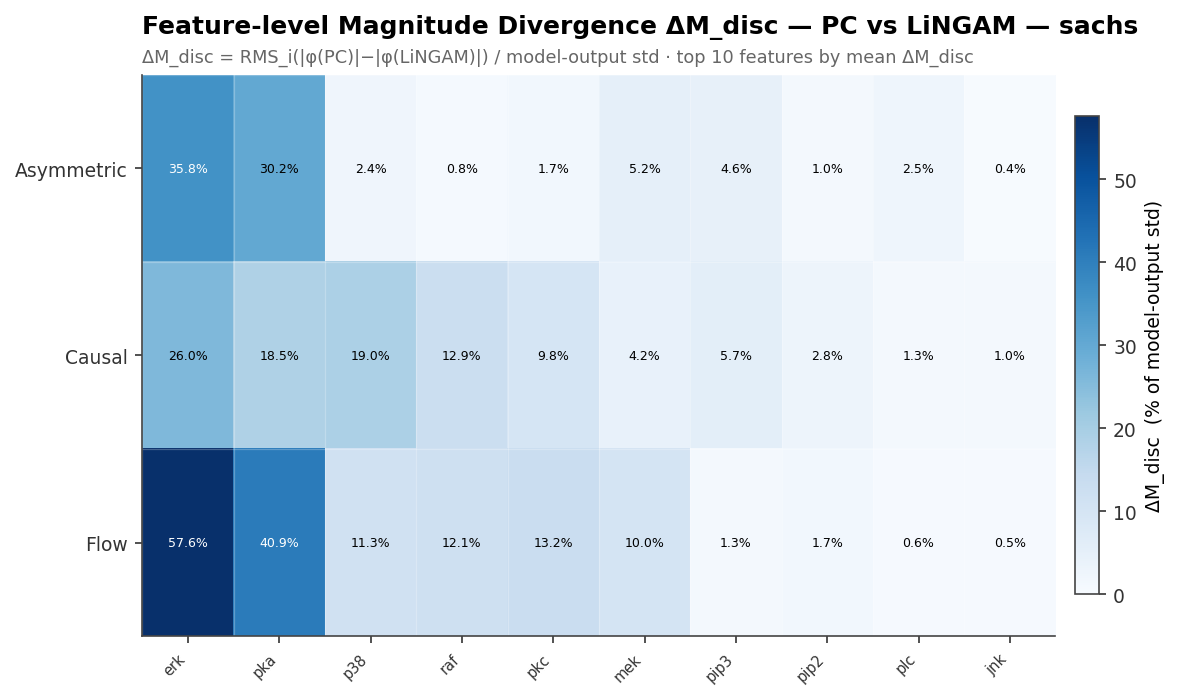
\includegraphics[width=\linewidth]{figures/gss_heatmap_sachs.png}
    \caption{Sachs. Sensitivity concentrates on erk and pka; Flow reaches
    57.5\% of $\hat{\sigma}$ on erk.}
    \label{fig:heatmap_disc_sachs}
  \end{subfigure}
  \caption{\textbf{Feature-level $\Delta M_{\text{disc}}$ (PC vs.\ LiNGAM).}}
  \label{fig:heatmap_disc}
\end{figure}

%% ============================================================
\subsection{Feature-Level Sign Disagreement Heatmaps ($D$)}
\label{app:heatmaps_sign}

Each heatmap shows $D^{\mathrm{ref}}_f$ for the top 10 features by mean sign
disagreement. Sign flips are qualitatively more damaging than magnitude shifts (they
invert the story told to the end user), and they tend to spread across more features
than magnitude changes because many near-zero attributions sit close to the sign
boundary.

\begin{figure}[H]
  \centering
  \begin{subfigure}[t]{0.48\linewidth}
    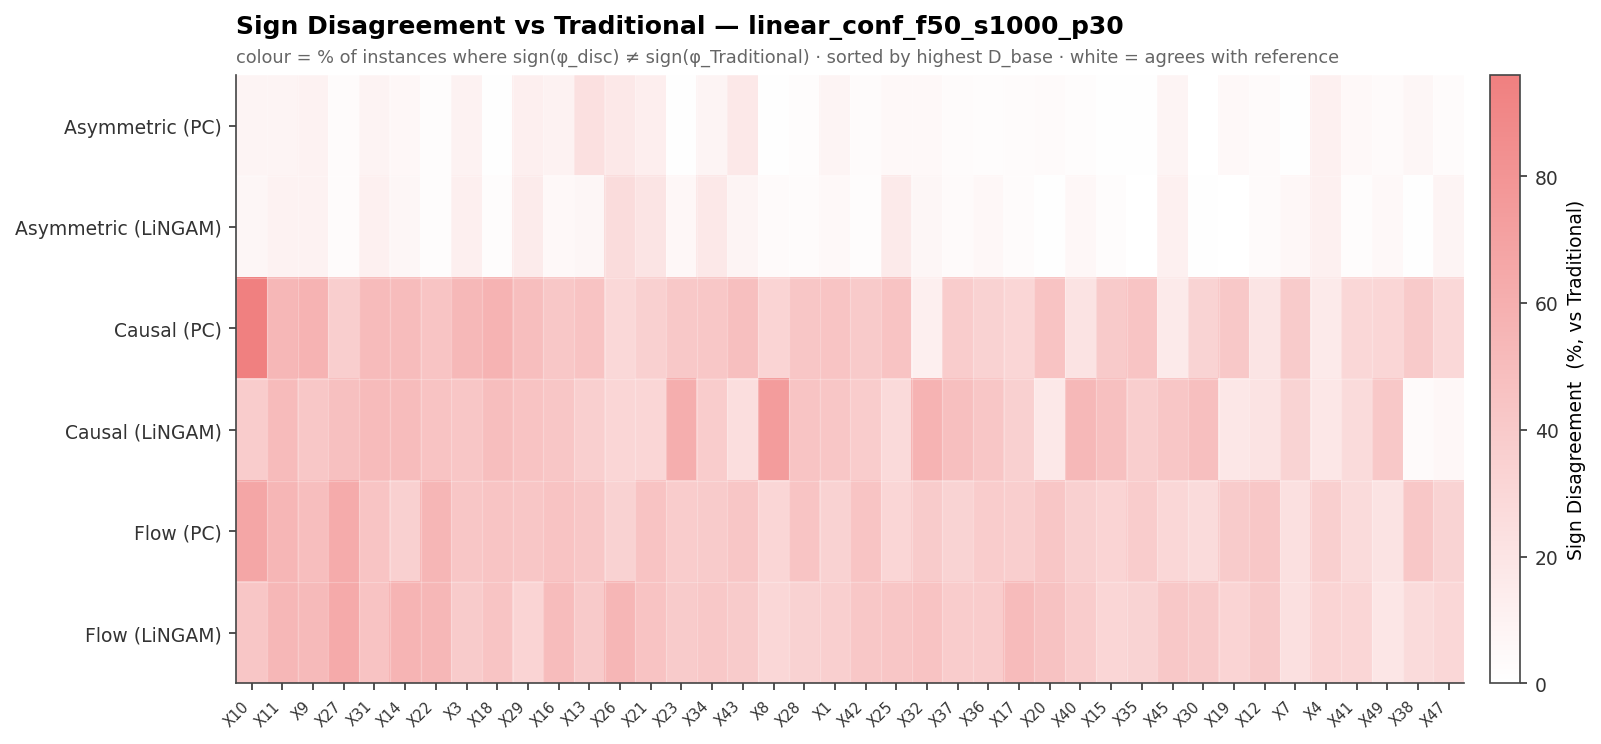
\includegraphics[width=\linewidth]{figures/sign_alignment_heatmap_traditional_linear_conf_f50_s1000_p30.png}
    \caption{Synthetic. Asymmetric rows near-zero; Causal and Flow concentrate
    sign flips on X24, X33, X47.}
    \label{fig:sign_trad_synth}
  \end{subfigure}
  \hfill
  \begin{subfigure}[t]{0.48\linewidth}
    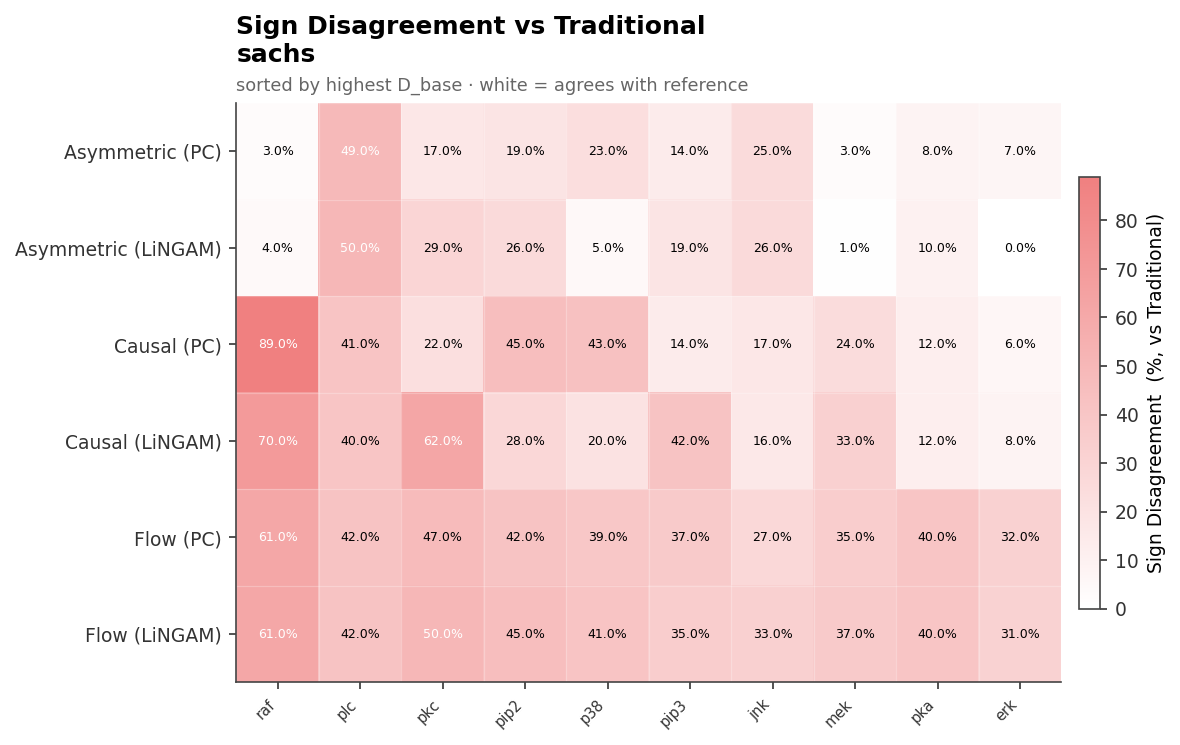
\includegraphics[width=\linewidth]{figures/sign_alignment_heatmap_traditional_sachs.png}
    \caption{Sachs. Sign disagreement concentrates on raf, plc, pkc; Causal+LiNGAM
    produces the highest per-feature flip rate vs.\ the baseline.}
    \label{fig:sign_trad_sachs}
  \end{subfigure}
  \caption{\textbf{Feature-level $D_{\text{base}}$ vs.\ Traditional Shapley.}}
  \label{fig:sign_trad}
\end{figure}

\begin{figure}[H]
  \centering
  \begin{subfigure}[t]{0.48\linewidth}
    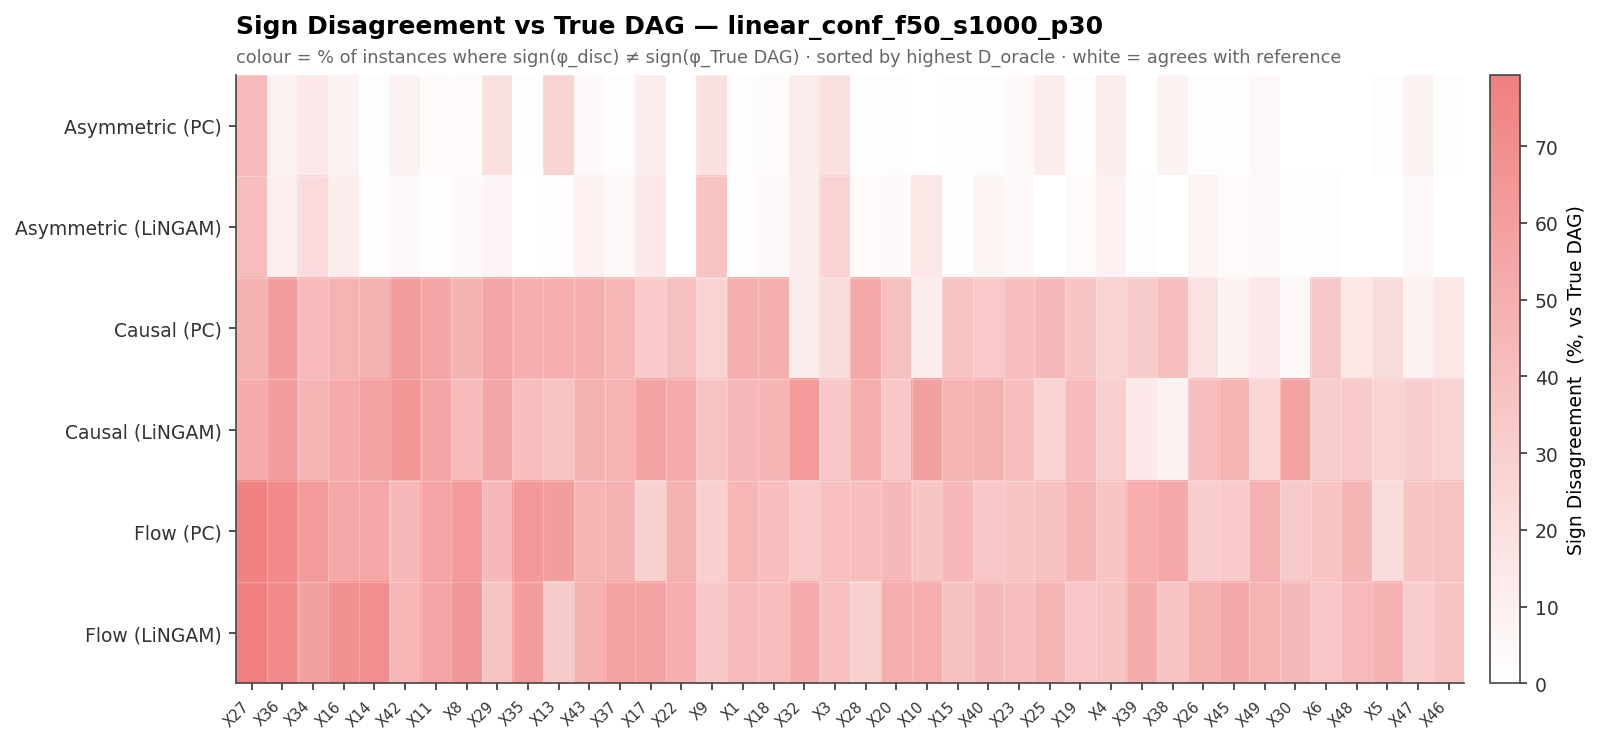
\includegraphics[width=\linewidth]{figures/sign_alignment_heatmap_true_linear_conf_f50_s1000_p30.png}
    \caption{Synthetic. Causal and Flow concentrate sign disagreement on X24,
    X33, X47, X6 --- the same features that carry the oracle magnitude deviations.}
    \label{fig:sign_oracle_synth}
  \end{subfigure}
  \hfill
  \begin{subfigure}[t]{0.48\linewidth}
    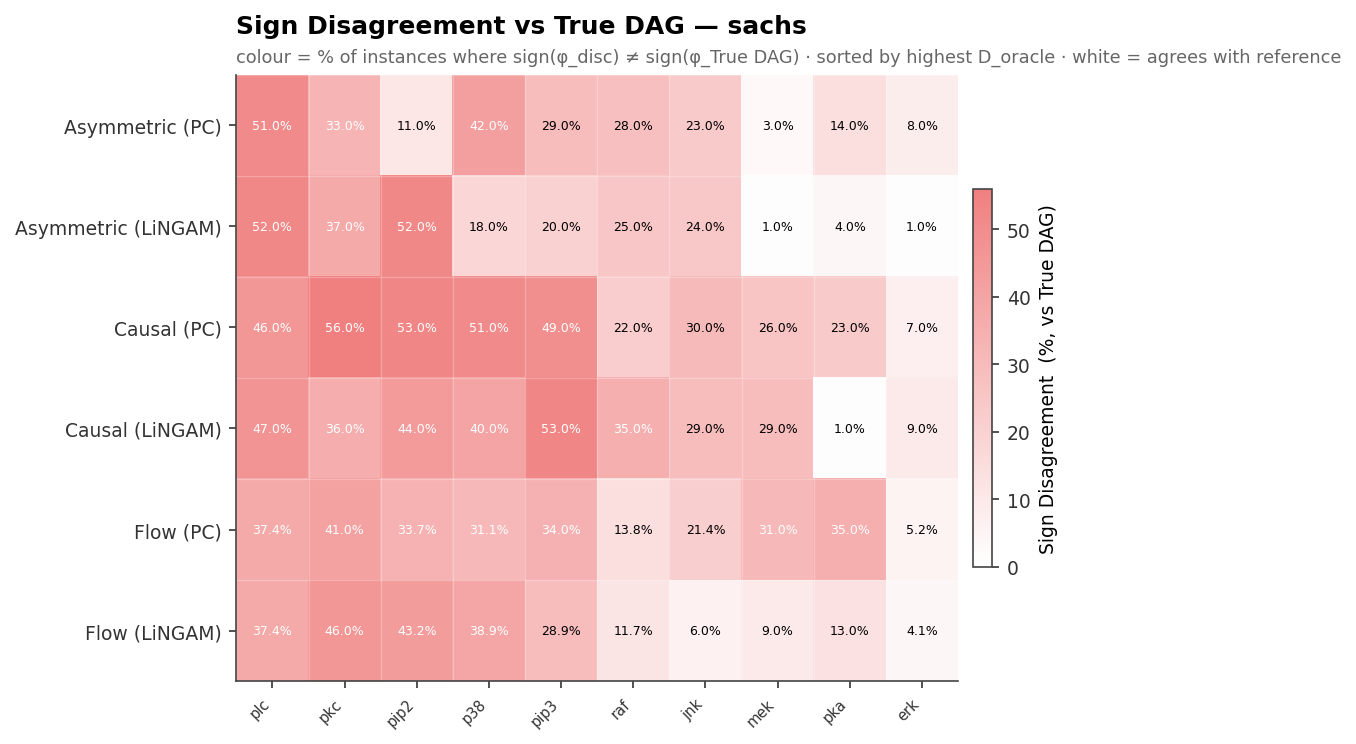
\includegraphics[width=\linewidth]{figures/sign_alignment_heatmap_true_sachs.png}
    \caption{Sachs. Sign disagreement vs.\ oracle concentrates on erk and pka;
    Flow+PC has the highest per-feature oracle sign-flip rate on erk.}
    \label{fig:sign_oracle_sachs}
  \end{subfigure}
  \caption{\textbf{Feature-level $D_{\text{oracle}}$ vs.\ the oracle DAG.}}
  \label{fig:sign_oracle}
\end{figure}

\begin{figure}[H]
  \centering
  \begin{subfigure}[t]{0.48\linewidth}
    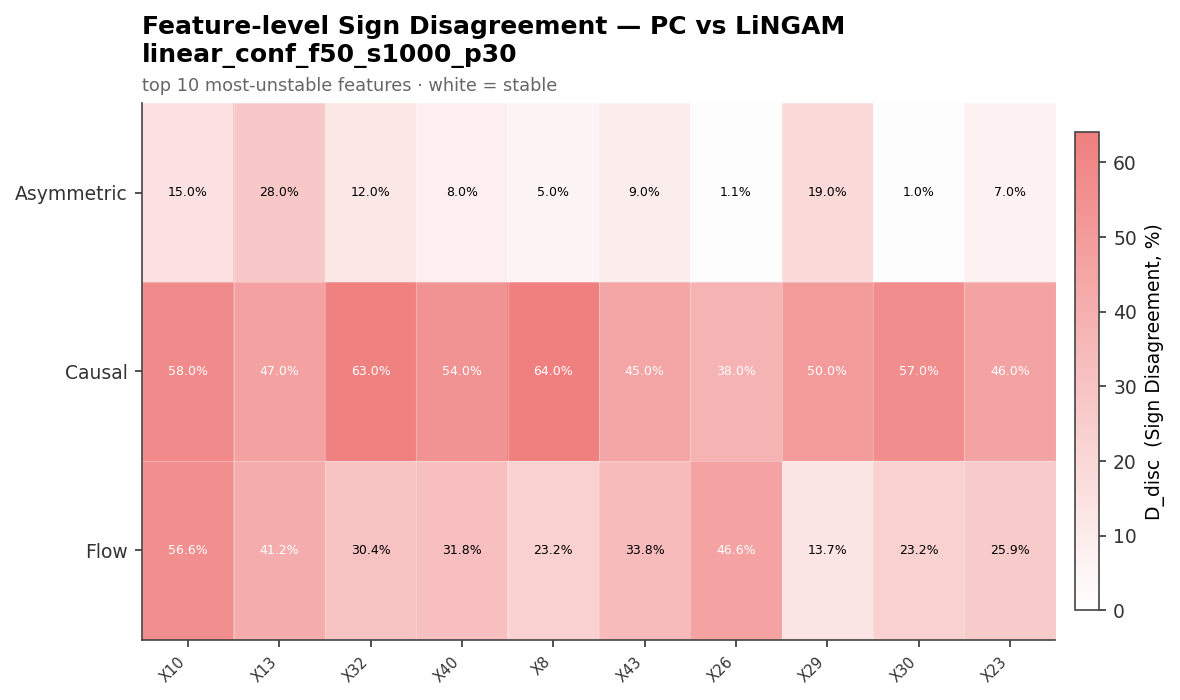
\includegraphics[width=\linewidth]{figures/sss_heatmap_linear_conf_f50_s1000_p30.png}
    \caption{Synthetic. Causal shows the highest sign instability concentrated on
    X10 and X32; Flow's sign instability is moderate vs.\ its magnitude sensitivity.}
    \label{fig:sign_disc_synth}
  \end{subfigure}
  \hfill
  \begin{subfigure}[t]{0.48\linewidth}
    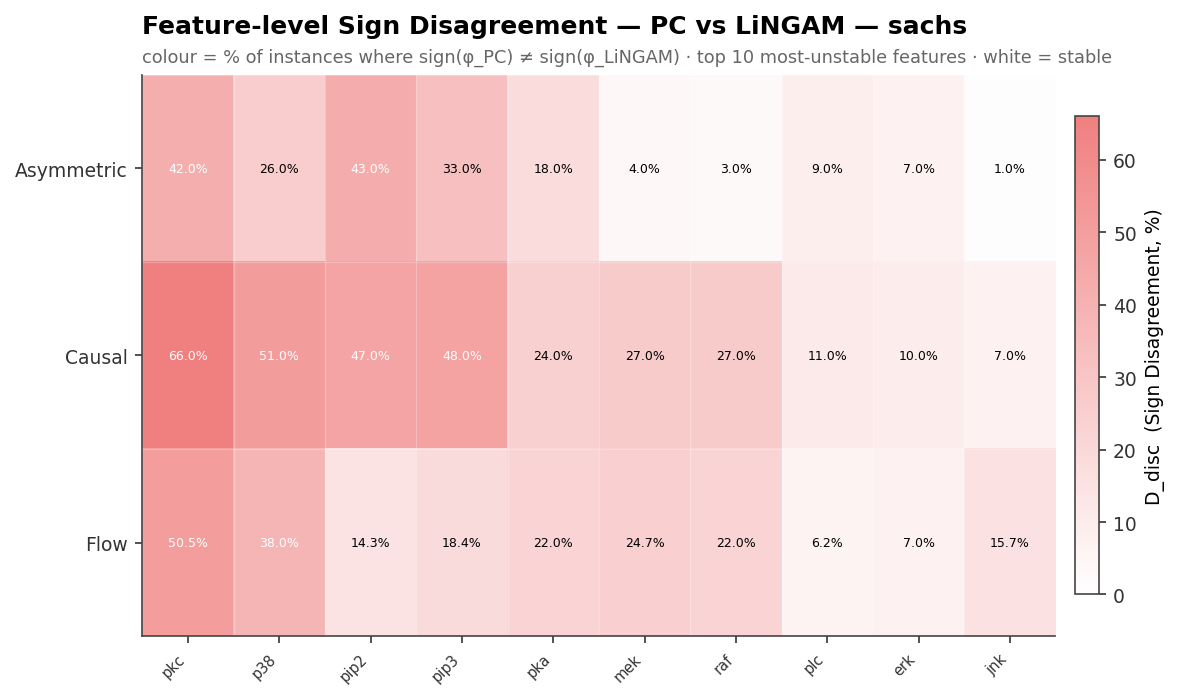
\includegraphics[width=\linewidth]{figures/sss_heatmap_sachs.png}
    \caption{Sachs. Sign instability concentrates on pkc and p38; Causal Shapley
    shows the broadest sign disagreement across proteins.}
    \label{fig:sign_disc_sachs}
  \end{subfigure}
  \caption{\textbf{Feature-level $D_{\text{disc}}$ (PC vs.\ LiNGAM).}}
  \label{fig:sign_disc}
\end{figure}

%% ============================================================
\section{Algorithm Pseudocode}
\label{app:algorithms}

The four main algorithms and five helper subroutines are listed below. They implement
the methods described in Section~\ref{sec:framework}.

\subsection{Main Methods}

\begin{algorithm}[H]
  \caption{Traditional Shapley (Monte Carlo)}
  \label{alg:traditional}
  \begin{algorithmic}[1]
    \INPUT{instance $x$, model $f$, background data $D$, permutations $T$}
    \OUTPUT{attribution vector $\phi \in \mathbb{R}^n$}
    \State $\phi \gets \mathbf{0}_n$;\quad $v_0 \gets \text{mean}(f(D))$
    \For{$t = 1 \ldots T$}
      \State $\pi \gets \textsc{random\_permutation}(1 \ldots n)$
      \State $S \gets \emptyset$;\quad $v_{\text{prev}} \gets v_0$
      \For{$i$ \textbf{in} $\pi$}
        \State $S \gets S \cup \{i\}$;\quad $v_{\text{curr}} \gets \textsc{coalition\_value}(x, S, f, D)$
        \State $\phi[i] \gets \phi[i] + (v_{\text{curr}} - v_{\text{prev}})$;\quad $v_{\text{prev}} \gets v_{\text{curr}}$
      \EndFor
    \EndFor
    \Return $\phi \mathbin{/} T$
  \end{algorithmic}
\end{algorithm}

\begin{algorithm}[H]
  \caption{Asymmetric Shapley}
  \label{alg:asymmetric}
  \begin{algorithmic}[1]
    \INPUT{instance $x$, model $f$, background $D$, feature DAG $G$, permutations $T$}
    \OUTPUT{attribution vector $\phi \in \mathbb{R}^n$}
    \PRECOMPUTE \texttt{children[]}, \texttt{in\_degree[]} from the $X$-only edges of $G$
    \State $\phi \gets \mathbf{0}_n$;\quad $v_0 \gets \text{mean}(f(D))$
    \For{$t = 1 \ldots T$}
      \State $\pi \gets \textsc{sample\_topological\_ordering}()$
      \State $S \gets \emptyset$;\quad $v_{\text{prev}} \gets v_0$
      \For{$i$ \textbf{in} $\pi$}
        \State $S \gets S \cup \{i\}$;\quad $v_{\text{curr}} \gets \textsc{coalition\_value}(x, S, f, D)$
        \State $\phi[i] \gets \phi[i] + (v_{\text{curr}} - v_{\text{prev}})$;\quad $v_{\text{prev}} \gets v_{\text{curr}}$
      \EndFor
    \EndFor
    \Return $\phi \mathbin{/} T$
  \end{algorithmic}
\end{algorithm}

\begin{algorithm}[H]
  \caption{Causal Shapley (post-interventional)}
  \label{alg:causal}
  \begin{algorithmic}[1]
    \INPUT{instance $x$, model $f$, background $D$, adjacency $A$ ($X$ only),
    confounder list, outer permutations $T$, inner samples $M$}
    \OUTPUT{attribution vector $\phi \in \mathbb{R}^n$}
    \PRECOMPUTE components, confounded[], parents[] $\gets$ \textsc{build\_components}$(A, \text{confounder list})$
    \State $\mu \gets \text{mean}(D)$;\quad $\Sigma \gets \text{cov}(D) + \varepsilon I$
    \State $\phi \gets \mathbf{0}_n$;\quad $v_0 \gets \text{mean}(f(D))$
    \For{$t = 1 \ldots T$}
      \State $\pi \gets \textsc{sample\_component\_topo\_ordering}()$, expand to features
      \State $S \gets \emptyset$;\quad $v_{\text{prev}} \gets v_0$
      \For{$i$ \textbf{in} $\pi$}
        \State $S \gets S \cup \{i\}$
        \State $v_{\text{curr}} \gets \frac{1}{M}\sum_{m=1}^{M} f\!\left(\textsc{post\_interventional\_sample}(x, S, \ldots)\right)$
        \State $\phi[i] \gets \phi[i] + (v_{\text{curr}} - v_{\text{prev}})$;\quad $v_{\text{prev}} \gets v_{\text{curr}}$
      \EndFor
    \EndFor
    \Return $\phi \mathbin{/} T$
  \end{algorithmic}
\end{algorithm}

\begin{algorithm}[H]
  \caption{Shapley Flow (uniform edge-permutation)}
  \label{alg:flow}
  \begin{algorithmic}[1]
    \INPUT{foreground instance $x_{\mathrm{fg}}$, background row $x_{\mathrm{bg}}$,
    graph adjacency ($n+1$ nodes incl.\ $Y$), target index $Y$, trials $T$}
    \OUTPUT{node attribution vector $\phi \in \mathbb{R}^n$ ($Y$ excluded)}
    \State $E \gets \text{list of all directed edges}$;\quad $\texttt{ec} \gets \{e: 0.0 \mid e \in E\}$
    \For{$t = 1 \ldots T$}
      \State $\text{perm} \gets \textsc{random\_permutation}(E)$;\quad $\text{active} \gets []$
      \State $v_{\text{prev}} \gets \textsc{system\_value}(\emptyset, x_{\mathrm{fg}}, x_{\mathrm{bg}})$
      \For{$e$ \textbf{in} perm}
        \State $\text{active.append}(e)$;\quad $v_{\text{curr}} \gets \textsc{system\_value}(\text{active}, x_{\mathrm{fg}}, x_{\mathrm{bg}})$
        \State $\texttt{ec}[e] \gets \texttt{ec}[e] + (v_{\text{curr}} - v_{\text{prev}})$;\quad $v_{\text{prev}} \gets v_{\text{curr}}$
      \EndFor
    \EndFor
    \State $\phi \gets \mathbf{0}_n$
    \For{each edge $(u \to v) \in E$ with $u \neq Y$}
      \State $\phi[u] \gets \phi[u] + \texttt{ec}[(u \to v)] \mathbin{/} T$
    \EndFor
    \Return $\phi$
  \end{algorithmic}
\end{algorithm}

\subsection{Subroutines}

\begin{algorithm}[H]
  \caption{COALITION\_VALUE --- $v(S) = \mathbb{E}[f(X) \mid X_S = x_S]$}
  \label{alg:coalition_value}
  \begin{algorithmic}[1]
    \Function{Coalition\_Value}{$x, S, f, D$}
      \State $\text{samples} \gets \text{copy}(D)$
      \For{each feature $j \in S$}
        \State $\text{samples}[:,j] \gets x[j]$
      \EndFor
      \Return $\text{mean}(f(\text{samples}))$
    \EndFunction
  \end{algorithmic}
\end{algorithm}

\begin{algorithm}[H]
  \caption{SAMPLE\_TOPOLOGICAL\_ORDERING --- uniform random linear extension (Kahn)}
  \label{alg:topo}
  \begin{algorithmic}[1]
    \PRECOMPUTE (once): \texttt{children[]}, \texttt{in\_degree[]} from the DAG ($Y$ excluded).
    \Statex \hspace{2.5em} If the feature DAG contains a cycle, disable constraints $\Rightarrow$ reduces to Traditional Shapley.
    \Function{Sample\_Topological\_Ordering}{\texttt{children}, \texttt{in\_degree}}
      \State $\text{deg} \gets \text{copy}(\texttt{in\_degree})$;\quad $\text{ready} \gets [i : \text{deg}[i] = 0]$;\quad $\text{order} \gets []$
      \While{$\text{ready} \neq \emptyset$}
        \State $\text{node} \gets \text{uniform pick from ready}$;\quad swap-remove from ready
        \State $\text{order.append(node)}$
        \For{$c \in \texttt{children}[\text{node}]$}
          \State $\text{deg}[c] \mathrel{-}= 1$;\quad \textbf{if} $\text{deg}[c] = 0$: $\text{ready.append}(c)$
        \EndFor
      \EndWhile
      \Return order
    \EndFunction
  \end{algorithmic}
\end{algorithm}

\begin{algorithm}[H]
  \caption{POST\_INTERVENTIONAL\_SAMPLE --- draw from $P(X \mid \mathrm{do}(X_S = x_S))$}
  \label{alg:post_int}
  \begin{algorithmic}[1]
    \Function{Post\_Interventional\_Sample}{$x, S$, components, confounded[], parents[], $\mu$, $\Sigma$}
      \State $\text{sample} \gets \mathbf{0}_n$;\quad \textbf{for} $j \in S$: $\text{sample}[j] \gets x[j]$
      \For{component $C$ in fixed topological order}
        \State $\text{missing} \gets C \setminus S$;\quad \textbf{if} $\text{missing} = \emptyset$: \textbf{continue}
        \If{\texttt{confounded}[$C$]}
          \For{$j \in \text{missing}$}
            \State $\text{sample}[j] \gets \textsc{gaussian\_conditional}(\{j\},\, \texttt{parents}[C],\, \mu,\, \Sigma)$
          \EndFor
        \Else
          \State $\text{sample}[\text{missing}] \gets \textsc{gaussian\_conditional}(\text{missing},\, \texttt{parents}[C] \cup (C \cap S),\, \mu,\, \Sigma)$
        \EndIf
      \EndFor
      \Return sample
    \EndFunction
  \end{algorithmic}
\end{algorithm}

\begin{algorithm}[H]
  \caption{GAUSSIAN\_CONDITIONAL --- closed-form conditional Gaussian draw}
  \label{alg:gaussian_cond}
  \begin{algorithmic}[1]
    \Function{Gaussian\_Conditional}{target $A$, cond $B$, vals $b$, $\mu$, $\Sigma$}
      \If{$B = \emptyset$}
        \Return draw from $\mathcal{N}(\mu_A,\, \Sigma_{AA})$
      \EndIf
      \State $\Sigma_{BB}^{-} \gets \textsc{pseudo\_inverse}(\Sigma_{BB})$
      \State $\mu_c \gets \mu_A + \Sigma_{AB}\,\Sigma_{BB}^{-}\,(b - \mu_B)$
      \State $\Sigma_c \gets \Sigma_{AA} - \Sigma_{AB}\,\Sigma_{BB}^{-}\,\Sigma_{BA}$;\quad symmetrise; nudge eigenvalues $\geq \varepsilon$
      \Return draw from $\mathcal{N}(\mu_c,\, \Sigma_c)$
    \EndFunction
  \end{algorithmic}
\end{algorithm}

\begin{algorithm}[H]
  \caption{SYSTEM\_VALUE --- binary foreground/background activation (Shapley Flow)}
  \label{alg:system_value}
  \begin{algorithmic}[1]
    \Function{System\_Value}{active\_edges, $x_{\mathrm{fg}}$, $x_{\mathrm{bg}}$}
      \For{each node $i$ in the graph}
        \If{($i$ is a source \textbf{and} has an active outgoing edge)
          \textbf{or} ($i$ has an active incoming edge)
          \textbf{or} (edge $i \to Y$ is active)}
          \State $\mathrm{val}[i] \gets x_{\mathrm{fg}}[i]$
        \Else
          \State $\mathrm{val}[i] \gets x_{\mathrm{bg}}[i]$
        \EndIf
      \EndFor
      \State drop $Y$ from val
      \Return $f(\mathrm{val})$
    \EndFunction
  \end{algorithmic}
\end{algorithm}

\end{document}
